\chapter{Style and Submission Requirements}

Requirements for other parts of the thesis work can be found on the school
web-pages~\cite{Noo05}.  The requirements below are for the written thesis
only.

\section{Format}
The following format specifications must be adhered to for your thesis
(the \LaTeX\ template available from the school ensures this):
\begin{enumerate}
\item The thesis must be written on \emph{A4 size paper}.
\item The thesis must be typed or prepared using a \emph{word-processor}.
\begin{itemize}
\item For Undergraduate theses, you are encouraged to use both sides
  of the paper.
\item For Higher Degree Research theses, your submitted thesis must be
   printed single-sided.
\end{itemize}
\item \emph{Margins} on all sides must be no less than \unit[20]{mm} (before
binding).
\item \emph{1.5 line spacing} (about \unit[8]{mm} per line) must be used.
\item All sheets must be \emph{numbered}. The main body of the thesis must be
numbered consecutively from beginning to end.  Other sections must either
be included or have their own logical numbering system.
\item The \emph{title page} must contain the following information:
\begin{enumerate}
\item University and School names.
\item Title of Thesis/Project.
\item Name of Author and student ID.
\item The degree the thesis is submitted for.
\item Submission date (month and year).
\item Supervisor's name (for undergraduate theses).
\end{enumerate}
\item After the body of the thesis, the thesis \emph{must} contain a
  Bibliography or References list as appropriate.

Authors should confer with their supervisors and School about the
style of their bibliography, as this varies between disciplines.
\end{enumerate}

\section{Other physical appearance}
Other requirements to the physical appearance of your theses are:
\begin{enumerate}
\item \emph{Graphs, diagrams and photographs} should be inserted as close as
possible to their \emph{first reference} in the text. Rotated
graphs etc are to be arranged so as to be conveniently read, with the
bottom edge to the outside of the page.
\emph{Graphs and diagrams must be legible!}
\item \emph{Supplementary material (for example CFD animations)} may be submitted either online or via external drive, and must be referred to within the text. The text should make sense without the supplementary material available. 
\end{enumerate}

\section{Submission}

Finally, here are some requirements to the submission procedure. 

\begin{enumerate}
\item The \emph{author} of the thesis is \emph{responsible} for the preparation of the
thesis before the deadline, proofreading the
typescript and having corrections made as necessary.
\item For undergraduate theses, there is a \emph{page limit} of 50 pages for the main body of the thesis.
\end{enumerate}



\chapter{Content Requirements}\label{ch:content}

Students should consult the literature (e.g.~\cite{Sid99,StrWhi79,Coo64,GRS14})
and other resources for material on how to write a good
thesis.  The present document is only a very brief introduction as to what
is expected.

\nocite{NieLeh03,HasLehKwo05}

\section{Structure}
Most theses are structured very much like the present document.
The main part of the thesis can be structured in many different ways,
however, but must contain: a \emph{problem definition};
\emph{theory} and \emph{considerations} on how to solve the problem;
a description of the \emph{solution method} (dimensioning, construction,
etc.);
presentation of \emph{results} (measurements, simulations, etc.);
a \emph{discussion} of the results (validity, deviations, comparison
with previous solutions, etc.); and finally the \emph{conclusions}.

\section{Style of writing}

\begin{enumerate}

\item Audience:
The thesis must be addressed to engineers at the same level as the
student but without the special knowledge gained during the thesis work.
Such a third-person must be able to reconstruct the results on the basis
of the thesis alone.

\item
Every used concept/symbol/abbreviation which is not widely know must be \emph{defined}.
The wording should be \emph{short} and \emph{concise}.  
Readable(!) \emph{figures} and \emph{graphs} enhances comprehensibility.

\item Units.
\emph{SI units} must be used.
\end{enumerate}

\section{Documentation}

\begin{enumerate}
\item
The work must be well documented; i.e. enclosed must be the \emph{complete
schematics} of designed electronic circuits/test set-ups and/or a
\emph{program listing}, and/or etc.
Documentation of \emph{simulation results} and/or \emph{measurement
results} likewise.
\item References:
For every declaration/equation/method/etc., which is not widely known,
a \emph{reference to the literature} must be given (or a `proof' if it is
the authors own work).
In case material is copied verbatim, quotes must be used.
This is also the case when referring to partners
work in the case of a Group Thesis.

\item Plagiarism:
Failure to give proper references to the literature is \emph{plagiarism}.
Plagiarism is considered serious offence and severe penalties may apply.

\end{enumerate}

\chapter{Project Plan}\label{ch:style}

% Include your planning for your feature here
\section{Topic Tree}
\subsection{Overview}
Most learning management systems do not have a simple and easy method to import course material and resources from other courses. Some LMS platforms such as OpenLearning have no method of importing any data at all, and other platforms such as Canvas allows you to import crowd sourced material into your own course, however still does not allow you to import topics of resources. \\

This new LMS has a new topic tree feature, which will allow teachers and academics to add course material under a specific topic instead.\\

\textbf{Topics} \\
A topic is a collection of educational material that is related to a particular subject. For example, in UNSW's Introduction to Programming course (COMP1511), one of the topics in the course is ``Pointers", which contains all course material related to pointers.\\

At Charles Sturt University, each topic is defined as a small subject that is three hours in length \cite{csutopictree}. CSU's curriculum covers around 1000 topics with each topic being three hours in length for a degree. In this thesis, we will also define a topic being three hours of content, but instructors can choose what amount of content constitutes as a topic.\\

\textbf{Topic Groups} \\
Topic groups are similar to courses themselves, except they are purely for organisational and enrolment purposes. We found that it would be much easier to enrol students into a group of topics instead of each individual topic, and it makes searching the topic tree much easier as there are a smaller number of topic groups than topics themselves. \\

Topic groups themselves do not contain assessments, exams, or any other resources. Only topics themselves contain this information. Therefore, academics must store assessments in individual topics and set up the prerequisites so if they wish, they can store a final exam in the last topic that students must complete or in an empty "milestone" topic. We decided to name this grouping of topics as "topic groups" instead of courses due to how a traditional course contains assessments and other content for the entire course, and does not have prerequisites between the topics themselves. This naming helps differentiate the system from the traditional university model.\\

\textbf{Prerequisites} \\

Each topic can have its own prerequisites, as discussed briefly previously. Some topics must be completed in order to complete the current topic. Prerequisites can be across topic groups as well. For example, Linked Lists in the "Introduction to Programming" topic group must be completed in order to start Graphs in "Data Structures and Algorithms". This improves reusability, as topics in other topic groups can be set as prerequisites eg. Git can be set a prerequisite for "Web Front end Programming" instead.

\textbf{Reusability} \\
The topic tree enables academics to easily reuse content - by setting specific topics, academics can reuse content instead of creating new content for the same topic in their own course. A good example of this is "Web Front end Programming" at UNSW - Instead of creating new content for Git, academics can set Git as a prerequisite. However, to encourage reusability, a cloning feature is also provided where academics can clone a topic and its resources from another topic group and put it in its own topic group. This further enables reusability, demonstrating that there is no need to spend time creating new content.\\

\textbf{Course Materials} \\
The Meta Learning Management System also organises content into four sections:
\begin{itemize}
    \item Content
    \item Practice
    \item Preparation
    \item Assessments
\end{itemize}

These various sections were chosen as they fit many learning models, including UNSW's learning models as listed on their website \cite{learningModel}. Students are introduced to it in the content section, and then get to know more about it in the practice section, and try it out in the preparation and assessments sections. After receiving feedback, this cycle repeats again.\\

\begin{figure}[h!]
    \centering
    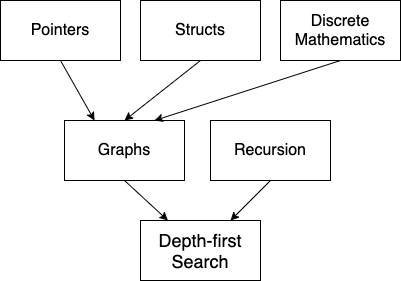
\includegraphics[scale=0.4]{topic-tree-example}
    \caption{Example of a topic tree with Depth first search}
\end{figure}

In the above example, pointers, structs and discrete mathematics must be learned in order to learn graphs. Likewise, graphs and recursion is required to learn depth first search.\\

\subsection{Initial Designs}
\begin{figure}[h!]
    \centering
    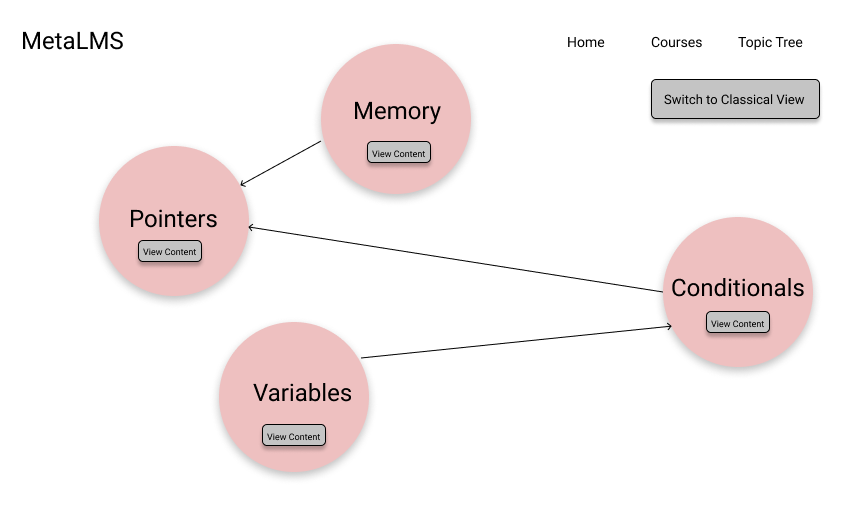
\includegraphics[scale=0.4]{topic-tree-graph-view}
    \caption{Topic Groups Graph UI}
\end{figure}

The above design is an initial design of the graph view of the topic tree. It was intended that there would only be topics when the topic tree was first designed, and the user could select a topic group to view the topic tree for that topic group. However, it was impossible to view prerequisites across topic groups with this design, and made it more difficult to view topics inside different topic groups. Therefore, a new design was chosen as follows.

\begin{figure}[h!]
    \centering
    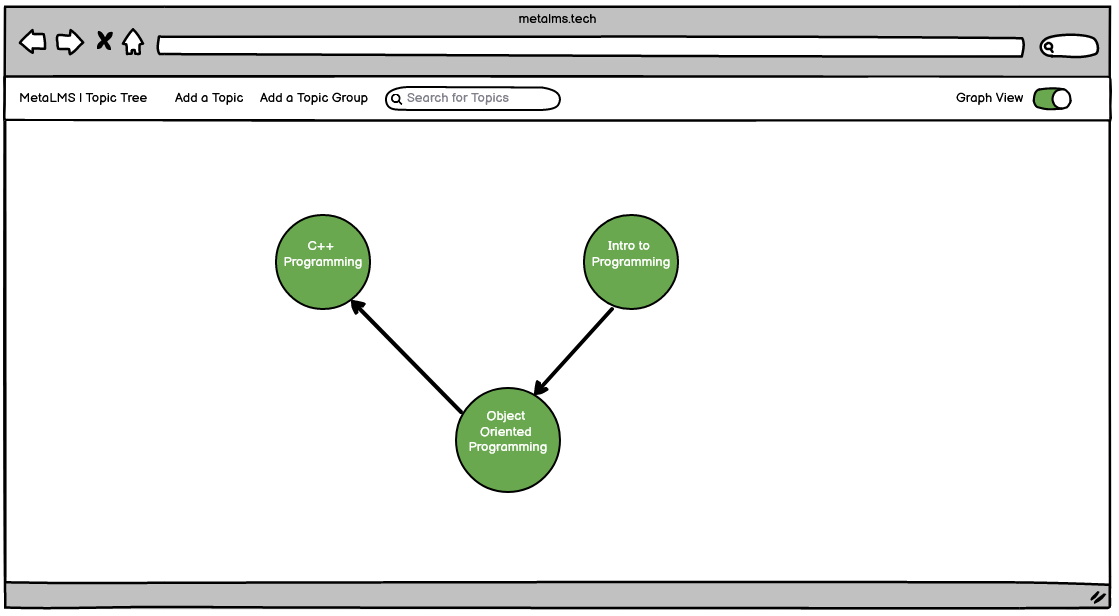
\includegraphics[scale=0.4]{topic-tree-graph-view-final-design}
    \caption{Topic Groups Graph UI Final Design}
\end{figure}

Instead, the topic groups are all shown on one graph, and a simple toggle to switch between the list view and the graph view is displayed in the top right. There are more options to add topic groups or topics at the top, and the user can click a topic group to show the individual topics as shown below.

\begin{figure}[h!]
    \centering
    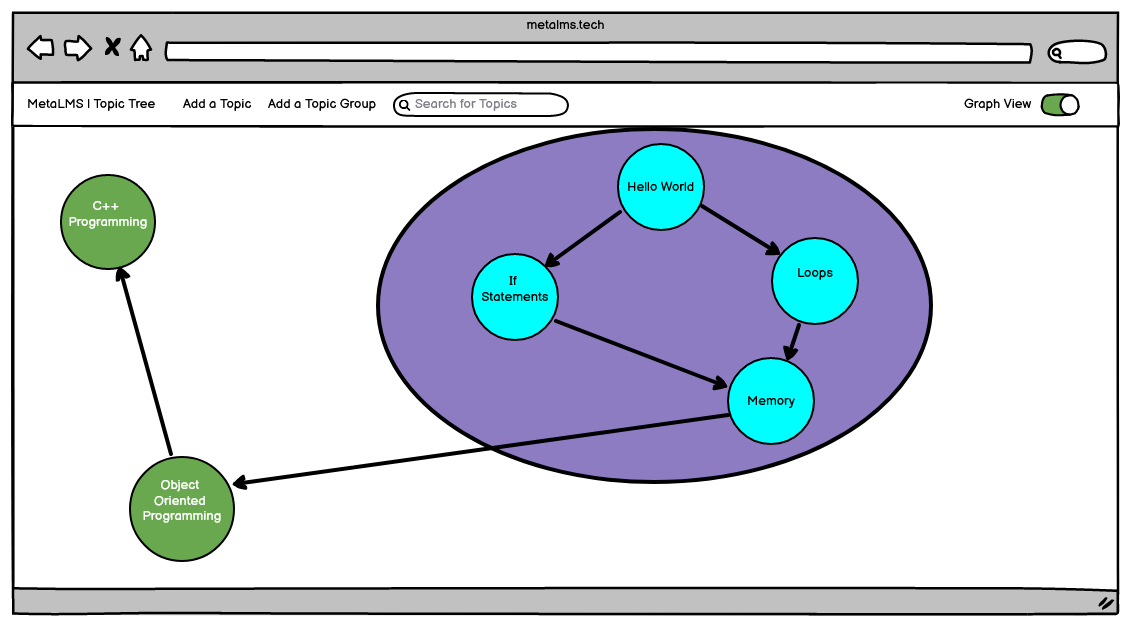
\includegraphics[scale=0.4]{topic-tree-expanded-design}
    \caption{Topic Groups Graph UI Expanded Topics}
\end{figure}

As shown, when a topic group is clicked, a hull in the background surrounds the topics to indicate they are part of the same group. Topics are shown in blue, and the individual prerequisites are shown with prerequisites pointing to topics in other topic groups as well. 

\begin{figure}[h!]
    \centering
    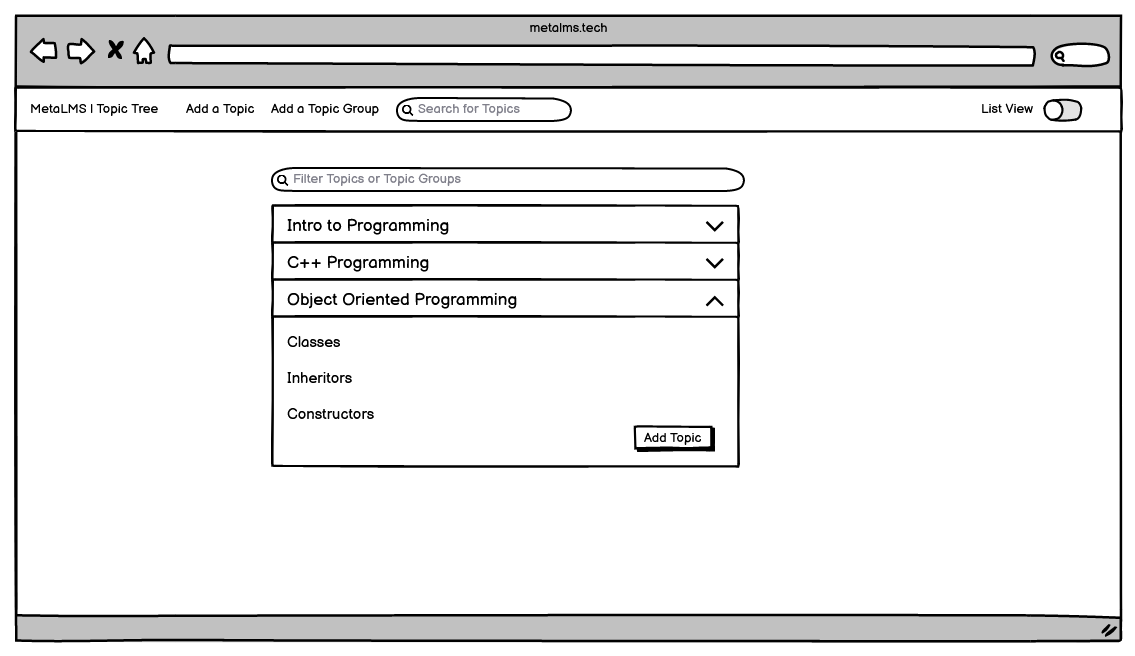
\includegraphics[scale=0.4]{topic-tree-list-view-final-design}
    \caption{Topic Groups List UI Final Design}
\end{figure}

As shown above, the final design of the list view shows both topics and topic groups on the same page to improve performance and usability, as there is less of a need to click through different pages to view different topic groups. Users can click on a specific topic group to expand and show the topics inside it, and click Add Topic to add a specific topic. Topics can be clicked to view their prerequisites.

\subsection{Requirements}
Each requirement will have a priority: High, Medium or Low. High priority requirements will be completed first, and then medium and low priority requirements respectively. \\

\subsection{Functional Requirements}

\textbf{Viewing Topics}

\begin{table}[hp]
\begin{tabular}{ll}
\textit{As a}      & User                                                \\ \hline
\textit{I want to} & View groups of topics                               \\ \hline
\textit{So that}   & I can see how topic groups interact with each other \\ \hline
\textit{Priority}  & {\color[HTML]{FE996B} Medium}                         \\ \hline
\textit{Status}    & Complete                                            \\ \hline
\end{tabular}
\end{table}

\begin{table}[hp]
\begin{tabular}{ll}
\textit{As a}      & User                                                \\ \hline
\textit{I want to} & View topics within each topic group                 \\ \hline
\textit{So that}   & I can see how topic groups interact with each other \\ \hline
\textit{Priority}  & {\color[HTML]{FE0000} High}                         \\ \hline
\textit{Status}    & Complete                                            \\ \hline
\end{tabular}
\end{table}

\begin{table}[hp]
\begin{tabular}{ll}
\textit{As a}      & User                                                \\ \hline
\textit{I want to} & View topics within each topic group                 \\ \hline
\textit{So that}   & I can see how topic groups interact with each other \\ \hline
\textit{Priority}  & {\color[HTML]{FE0000} High}                         \\ \hline
\textit{Status}    & Complete                                            \\ \hline
\end{tabular}
\end{table}

\begin{table}[hp]
\begin{tabular}{ll}
\textit{As a}      & User                                                           \\ \hline
\textit{I want to} & Search for specific resources                                  \\ \hline
\textit{So that}   & I can find other resources easily in the many topics available \\ \hline
\textit{Priority}  & {\color[HTML]{FE0000} High}                                    \\ \hline
\textit{Status}    & Not Complete                                                   \\ \hline          
\end{tabular}
\end{table}

\begin{table}[hp]
\begin{tabular}{ll}
\textit{As a}      & User                                                                            \\ \hline
\textit{I want to} & View topic prerequisites                                                        \\ \hline
\textit{So that}   & I can see which topics must be completed in order to complete the current topic \\ \hline
\textit{Priority}  & {\color[HTML]{FE996B} Medium}                                                     \\ \hline
\textit{Status}    & Complete                                                                        \\ \hline                              
\end{tabular}
\end{table}

\begin{table}[hp]
\begin{tabular}{ll}
\textit{As a}      & User                                                   \\ \hline
\textit{I want to} & view a graph of topics and their prerequisites         \\ \hline
\textit{So that}   & The topics and their prerequisites are easily viewable \\ \hline
\textit{Priority}  & {\color[HTML]{FE0000} High}                            \\ \hline
\textit{Status}    & Complete                                               \\ \hline      
\end{tabular}
\end{table}

\begin{table}[hp]
\begin{tabular}{ll}
\textit{As a}      & User                                                              \\ \hline
\textit{I want to} & view the topic tree with a traditional interface                  \\ \hline
\textit{So that}   & topics can be viewed more easily using a less confusing interface \\ \hline
\textit{Priority}  & {\color[HTML]{3166FF} Low}                                        \\ \hline
\textit{Status}    & Complete                                                          \\ \hline
\end{tabular}
\end{table}

\textbf{Adding Topics and resources}
\begin{table}[hp]
\begin{tabular}{ll}
\textit{As a}      & User                                           \\ \hline
\textit{I want to} & add a new topic                                \\ \hline
\textit{So that}   & I can edit the topic tree and add more content \\ \hline
\textit{Priority}  & {\color[HTML]{FE0000} High}                    \\ \hline
\textit{Status}    & Complete                                       \\ \hline              
\end{tabular}
\end{table}

\begin{table}[hp]
\begin{tabular}{ll}
\textit{As a}      & Academic                       \\ \hline
\textit{I want to} & upload course material      \\ \hline
\textit{So that}   & I can add content to topics       \\ \hline
\textit{Priority}  & {\color[HTML]{FE0000} High} \\ \hline
\textit{Status}    & Complete                    \\ \hline 
\end{tabular}
\end{table}

\begin{table}[hp]
\begin{tabular}{|l|l|}
\hline
\textit{As a}      & Academic                                                                      \\ \hline
\textit{I want to} & add a new topic group                                                     \\ \hline
\textit{So that}   & topics are more organised and I can create new topics under the new group \\ \hline
\textit{Priority}  & {\color[HTML]{F8A102} Medium}                                             \\ \hline
\textit{Status}    & Complete                                                                  \\ \hline
\end{tabular}
\end{table}

\begin{table}[hp]
\begin{tabular}{|l|l|}
\hline
\textit{As a}      & Academic                                 \\ \hline
\textit{I want to} & Add tags to a topic                      \\ \hline
\textit{So that}   & Search for topics faster and more easily \\ \hline
\textit{Priority}  & {\color[HTML]{3531FF} Low}               \\ \hline
\textit{Status}    & Complete                                 \\ \hline
\end{tabular}
\end{table}

\begin{table}[hp]
\begin{tabular}{|l|l|}
\hline
\textit{As a}      & Academic                                                                      \\ \hline
\textit{I want to} & add a new topic group                                                     \\ \hline
\textit{So that}   & topics are more organised and I can create new topics under the new group \\ \hline
\textit{Priority}  & {\color[HTML]{F8A102} Medium}                                             \\ \hline
\textit{Status}    & Complete                                                                  \\ \hline
\end{tabular}
\end{table}

\textbf{Deleting Topics}

\begin{table}[hp]
\begin{tabular}{|l|l|}
\hline
\textit{As a}      & Academic                                 \\ \hline
\textit{I want to} & delete a topic that I've created         \\ \hline
\textit{So that}   & I can remove content from the topic tree \\ \hline
\textit{Priority}  & {\color[HTML]{FE0000} High}              \\ \hline
\textit{Status}    & Complete                                 \\ \hline
\end{tabular}
\end{table}

\begin{table}[hp]
\begin{tabular}{|l|l|}
\hline
\textit{As a}      & Academic                                 \\ \hline
\textit{I want to} & delete a topic group that I've created   \\ \hline
\textit{So that}   & I can remove content from the topic tree \\ \hline
\textit{Priority}  & {\color[HTML]{F8A102} Medium}              \\ \hline
\textit{Status}    & Not Complete                                 \\ \hline
\end{tabular}
\end{table}

\begin{table}[hp]
\begin{tabular}{|l|l|}
\hline
\textit{As a}      & Academic                                                    \\ \hline
\textit{I want to} & remove course material from a topic                         \\ \hline
\textit{So that}   & I can remove content from the topic tree that is not needed \\ \hline
\textit{Priority}  & {\color[HTML]{FE0000} High}                                 \\ \hline
\textit{Status}    & Complete                                                    \\ \hline
\end{tabular}
\end{table}

\textbf{Topic Prequisites}

\begin{table}[hp]
\begin{tabular}{|l|l|}
\hline
\textit{As a}      & Academic                                                                               \\ \hline
\textit{I want to} & add a topic prerequisite                                                               \\ \hline
\textit{So that}   & I can require other topics to be completed before students can learn the current topic \\ \hline
\textit{Priority}  & {\color[HTML]{FE996B} Medium}                                                            \\ \hline
\textit{Status}    & Complete                                                                               \\ \hline
\end{tabular}
\end{table}

\begin{table}[hp]
\begin{tabular}{|l|l|}
\hline
\textit{As a}      & Academic                                                                               \\ \hline
\textit{I want to} & delete a topic prerequisite                                                            \\ \hline
\textit{So that}   & I can remove requirements for a topic \\ \hline
\textit{Priority}  & {\color[HTML]{FE996B} Medium}                                                          \\ \hline
\textit{Status}    & Complete                                                                               \\ \hline
\end{tabular}
\end{table}

\textbf{Integration}

\begin{table}[hp]
\begin{tabular}{|l|l|}
\hline
\textit{As a}      & Academic                                                  \\ \hline
\textit{I want to} & allow third party integration such as YouTube and The Box \\ \hline
\textit{So that}   & I can use external services with the topic tree           \\ \hline
\textit{Priority}  & {\color[HTML]{3531FF} Low}                                \\ \hline
\textit{Status}    & Not Complete                                              \\ \hline
\end{tabular}
\end{table}

\textbf{Exporting}

\begin{table}[hp]
\begin{tabular}{|l|l|}
\hline
\textit{As a}      & Academic                                          \\ \hline
\textit{I want to} & Export data from topics and course material       \\ \hline
\textit{So that}   & I can use the topic tree data with other services \\ \hline
\textit{Priority}  & {\color[HTML]{3531FF} Low}                        \\ \hline
\textit{Status}    & Not Complete                                      \\ \hline
\end{tabular}
\end{table}

\subsection{Non Functional requirements}
The feature also has non functional requirements in order to better evaluate the completion of the feature. \\

\textbf{Performance} \\
Performance must be high and the feature must be responsive to provide a high quality user experience for both academics and students. Performance will be assessed using tools such as Google Lighthouse \cite{googleLighthouse}. Google Lighthouse uses several metrics to assess performance, as explained previously. \\

\textbf{Accessibility} \\
The topic tree feature will also be assessed on how accessible the interface is. If features such as alt tags, high contrast colours and keyboard navigation are not implemented then not all academics and students will be able to use the topic tree feature. Therefore, tools such as Google Lighthouse will be used to access its accessibility as the tool also includes metrics for measuring accessibility of a website \cite{googleLighthouseAccessibility}. \\

\textbf{Usability} \\
Finally, the feature will be assessed on its usability. This includes whether the topic tree feature is attractive and easy to use. Various students and academics will be surveyed on how easy they found the system to use. The number of errors and time taken to complete a task will also be assessed.\\

\subsection {Changes from inital requirements}

The initial requirements did not mention anything about third party integration such as integrating YouTube and The Box. Later, it was realised that third party services would be very useful in uploading files and managing content, and so the requirement was added.\\

Originally, the requirements also stated that there should be functionality to upload course material by selecting multiple topics. This did not make sense in the context of the topic tree, as course material is attached to specific topics, not topic groups, and so was removed from the final requirements.\\

Finally, tags were added to the final requirements. The searchability of the topic tree proved a difficult problem to solve, and by adding tags to topics, users would be able to search specific topics by their tags instead of by name. This was then added to the list of requirements as it greatly improved the searchability of the topic tree.\\
\section{Forums}
\subsection{Overview}
Forums are a common feature in learning management systems as it provides a community environment where students can ask questions and discuss content with educators and other students.
Many of these built-in forums, however, are very basic and lack sufficient search, sorting and filtering functionality.
In many cases, educators are turning to external, third-party forums in order to take advantage of the more advanced features that they offer.

The aim of this feature is to develop a built-in forum that meets students' and educators' needs so that they no longer need to use an external application.

The forum interface consists of the overview page and the individual post pages.

\newpage

\subsubsection{Forum Overview Page}

\begin{figure}[h!]
    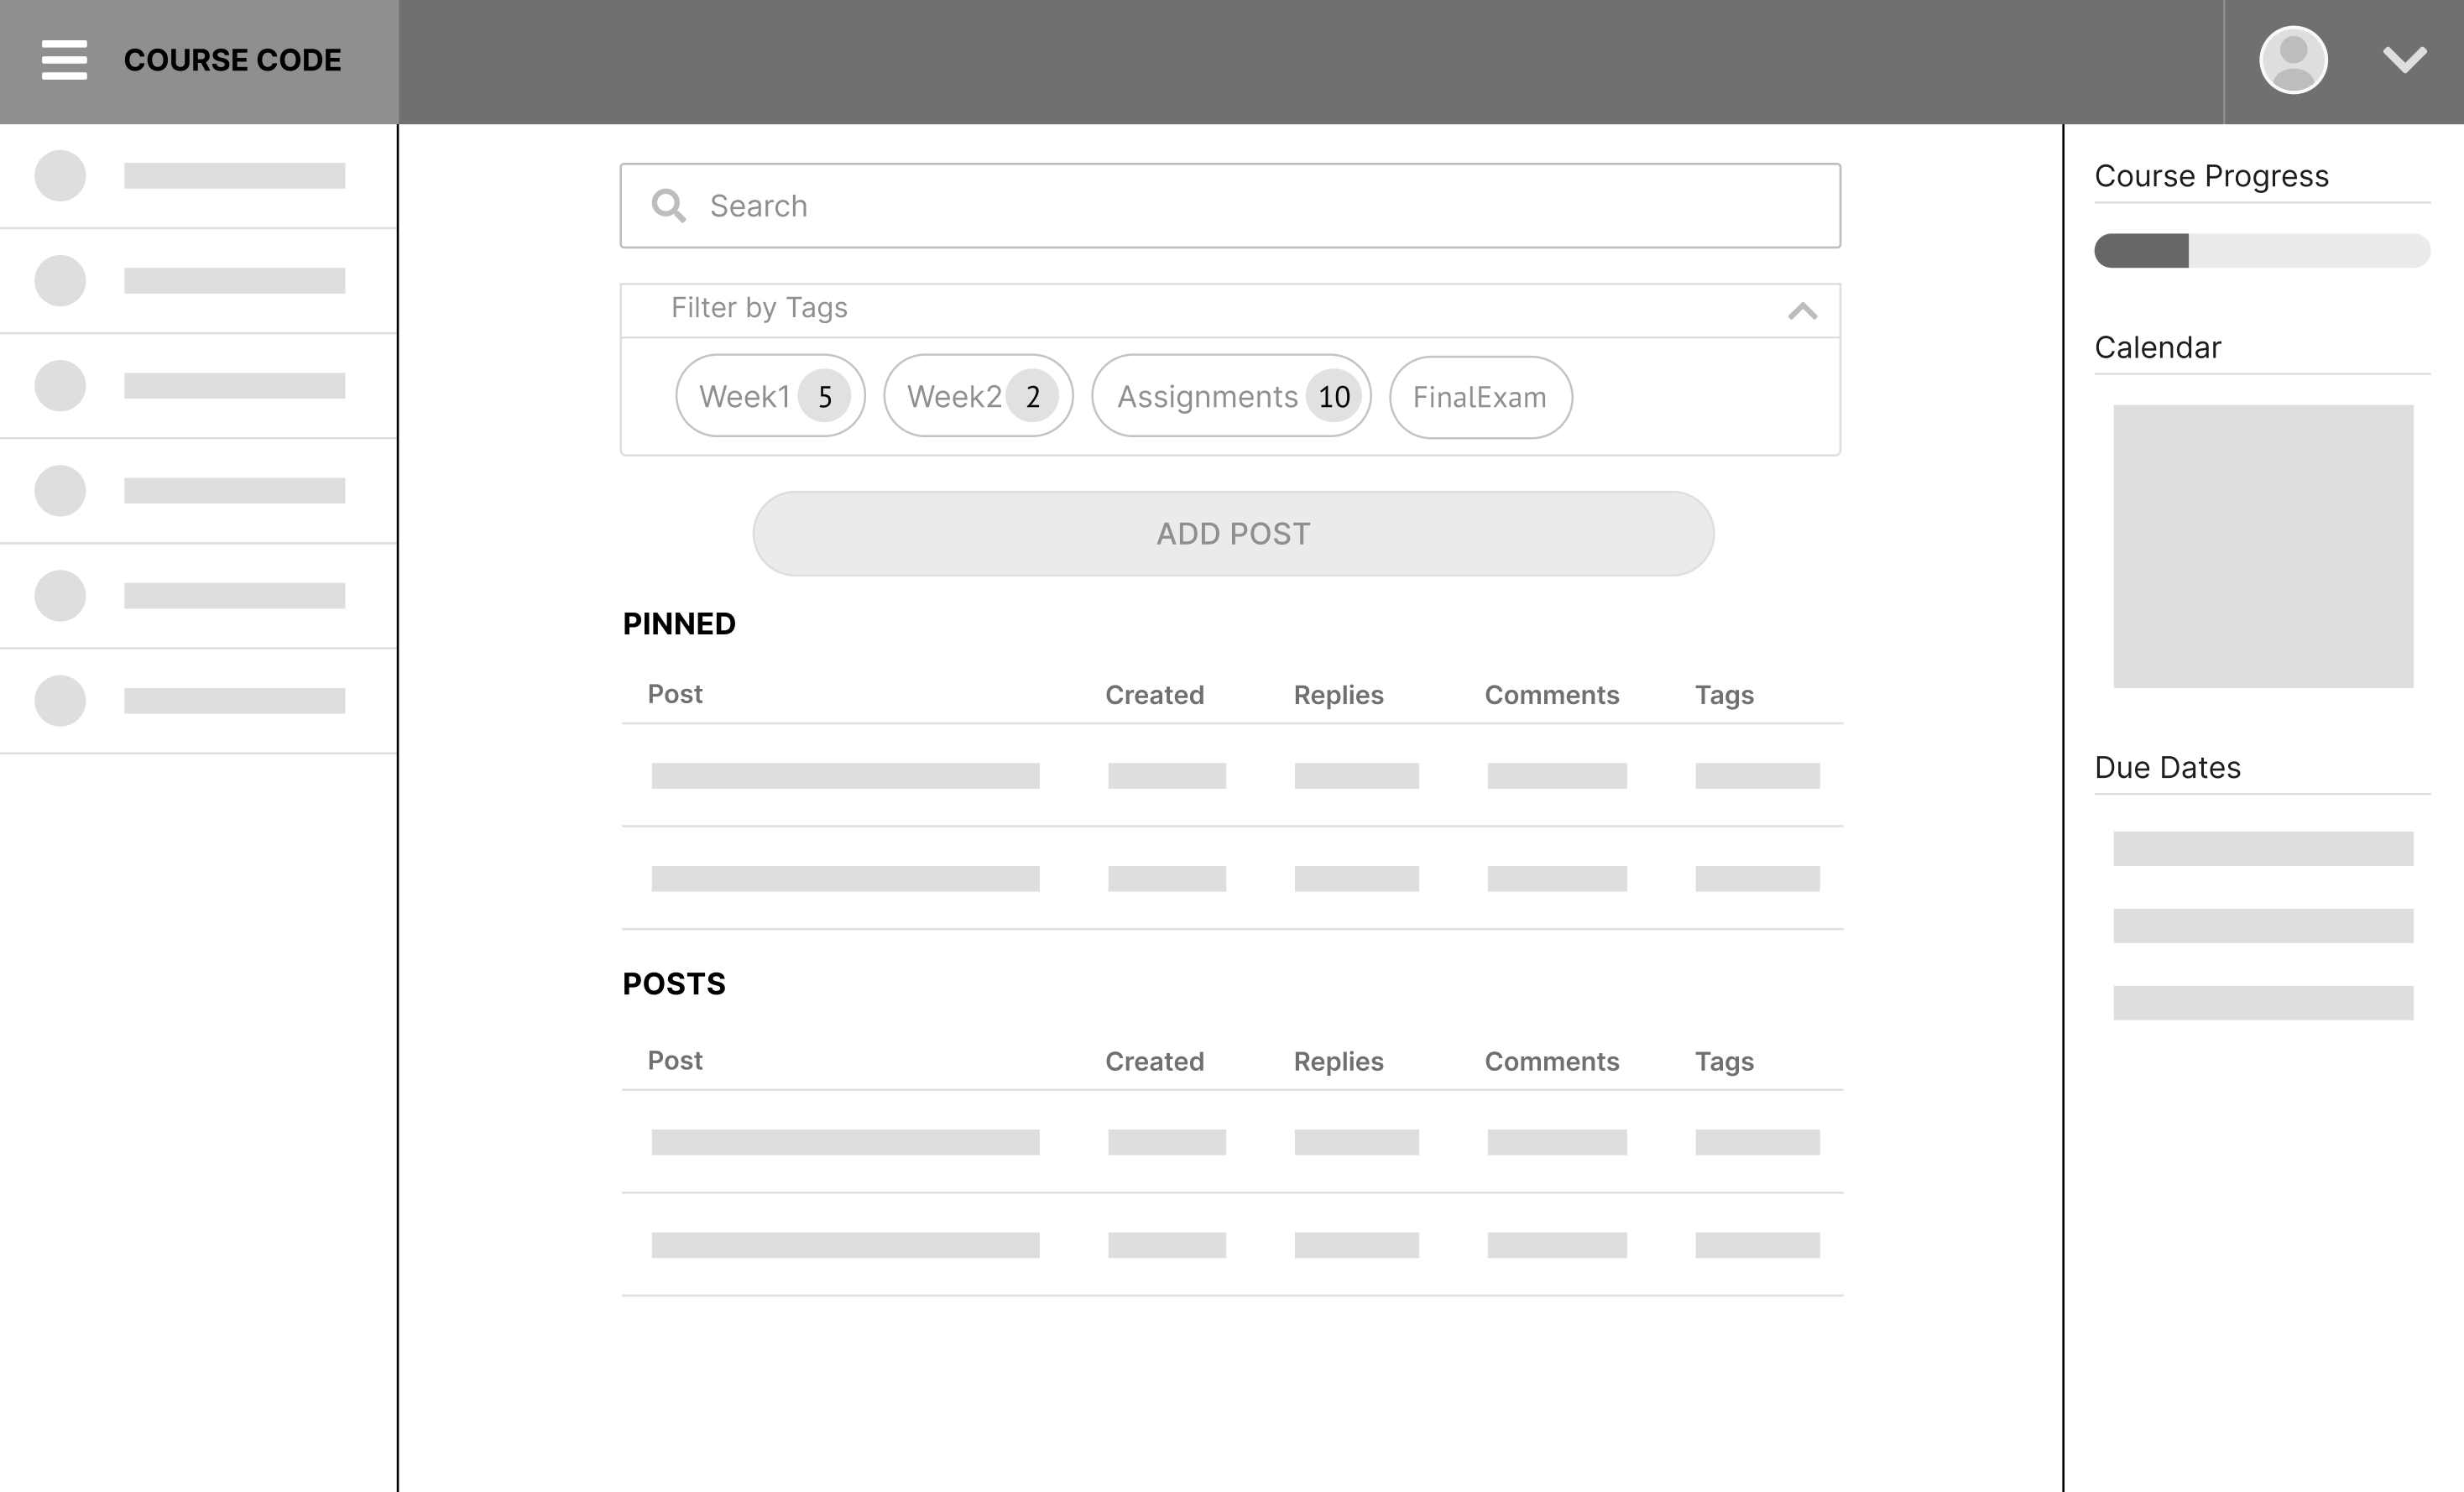
\includegraphics[scale=0.2]{forum-overview-page-student.png}
    \centering
    \caption{Forum overview page for a student}
\end{figure}

In general, the forum overview page consists of a list of posts, as well as search and filtering mechanisms.
The collapsible filter menu allows users to filter the forum post based on pre-defined tags.
Forum posts are ordered such that the list of pinned posts are at the top, followed by the remaining posts in chronological order.
Each row in the table includes the post title, date created, number of replies, number of comments and the associated tags.

\begin{figure}[h!]
    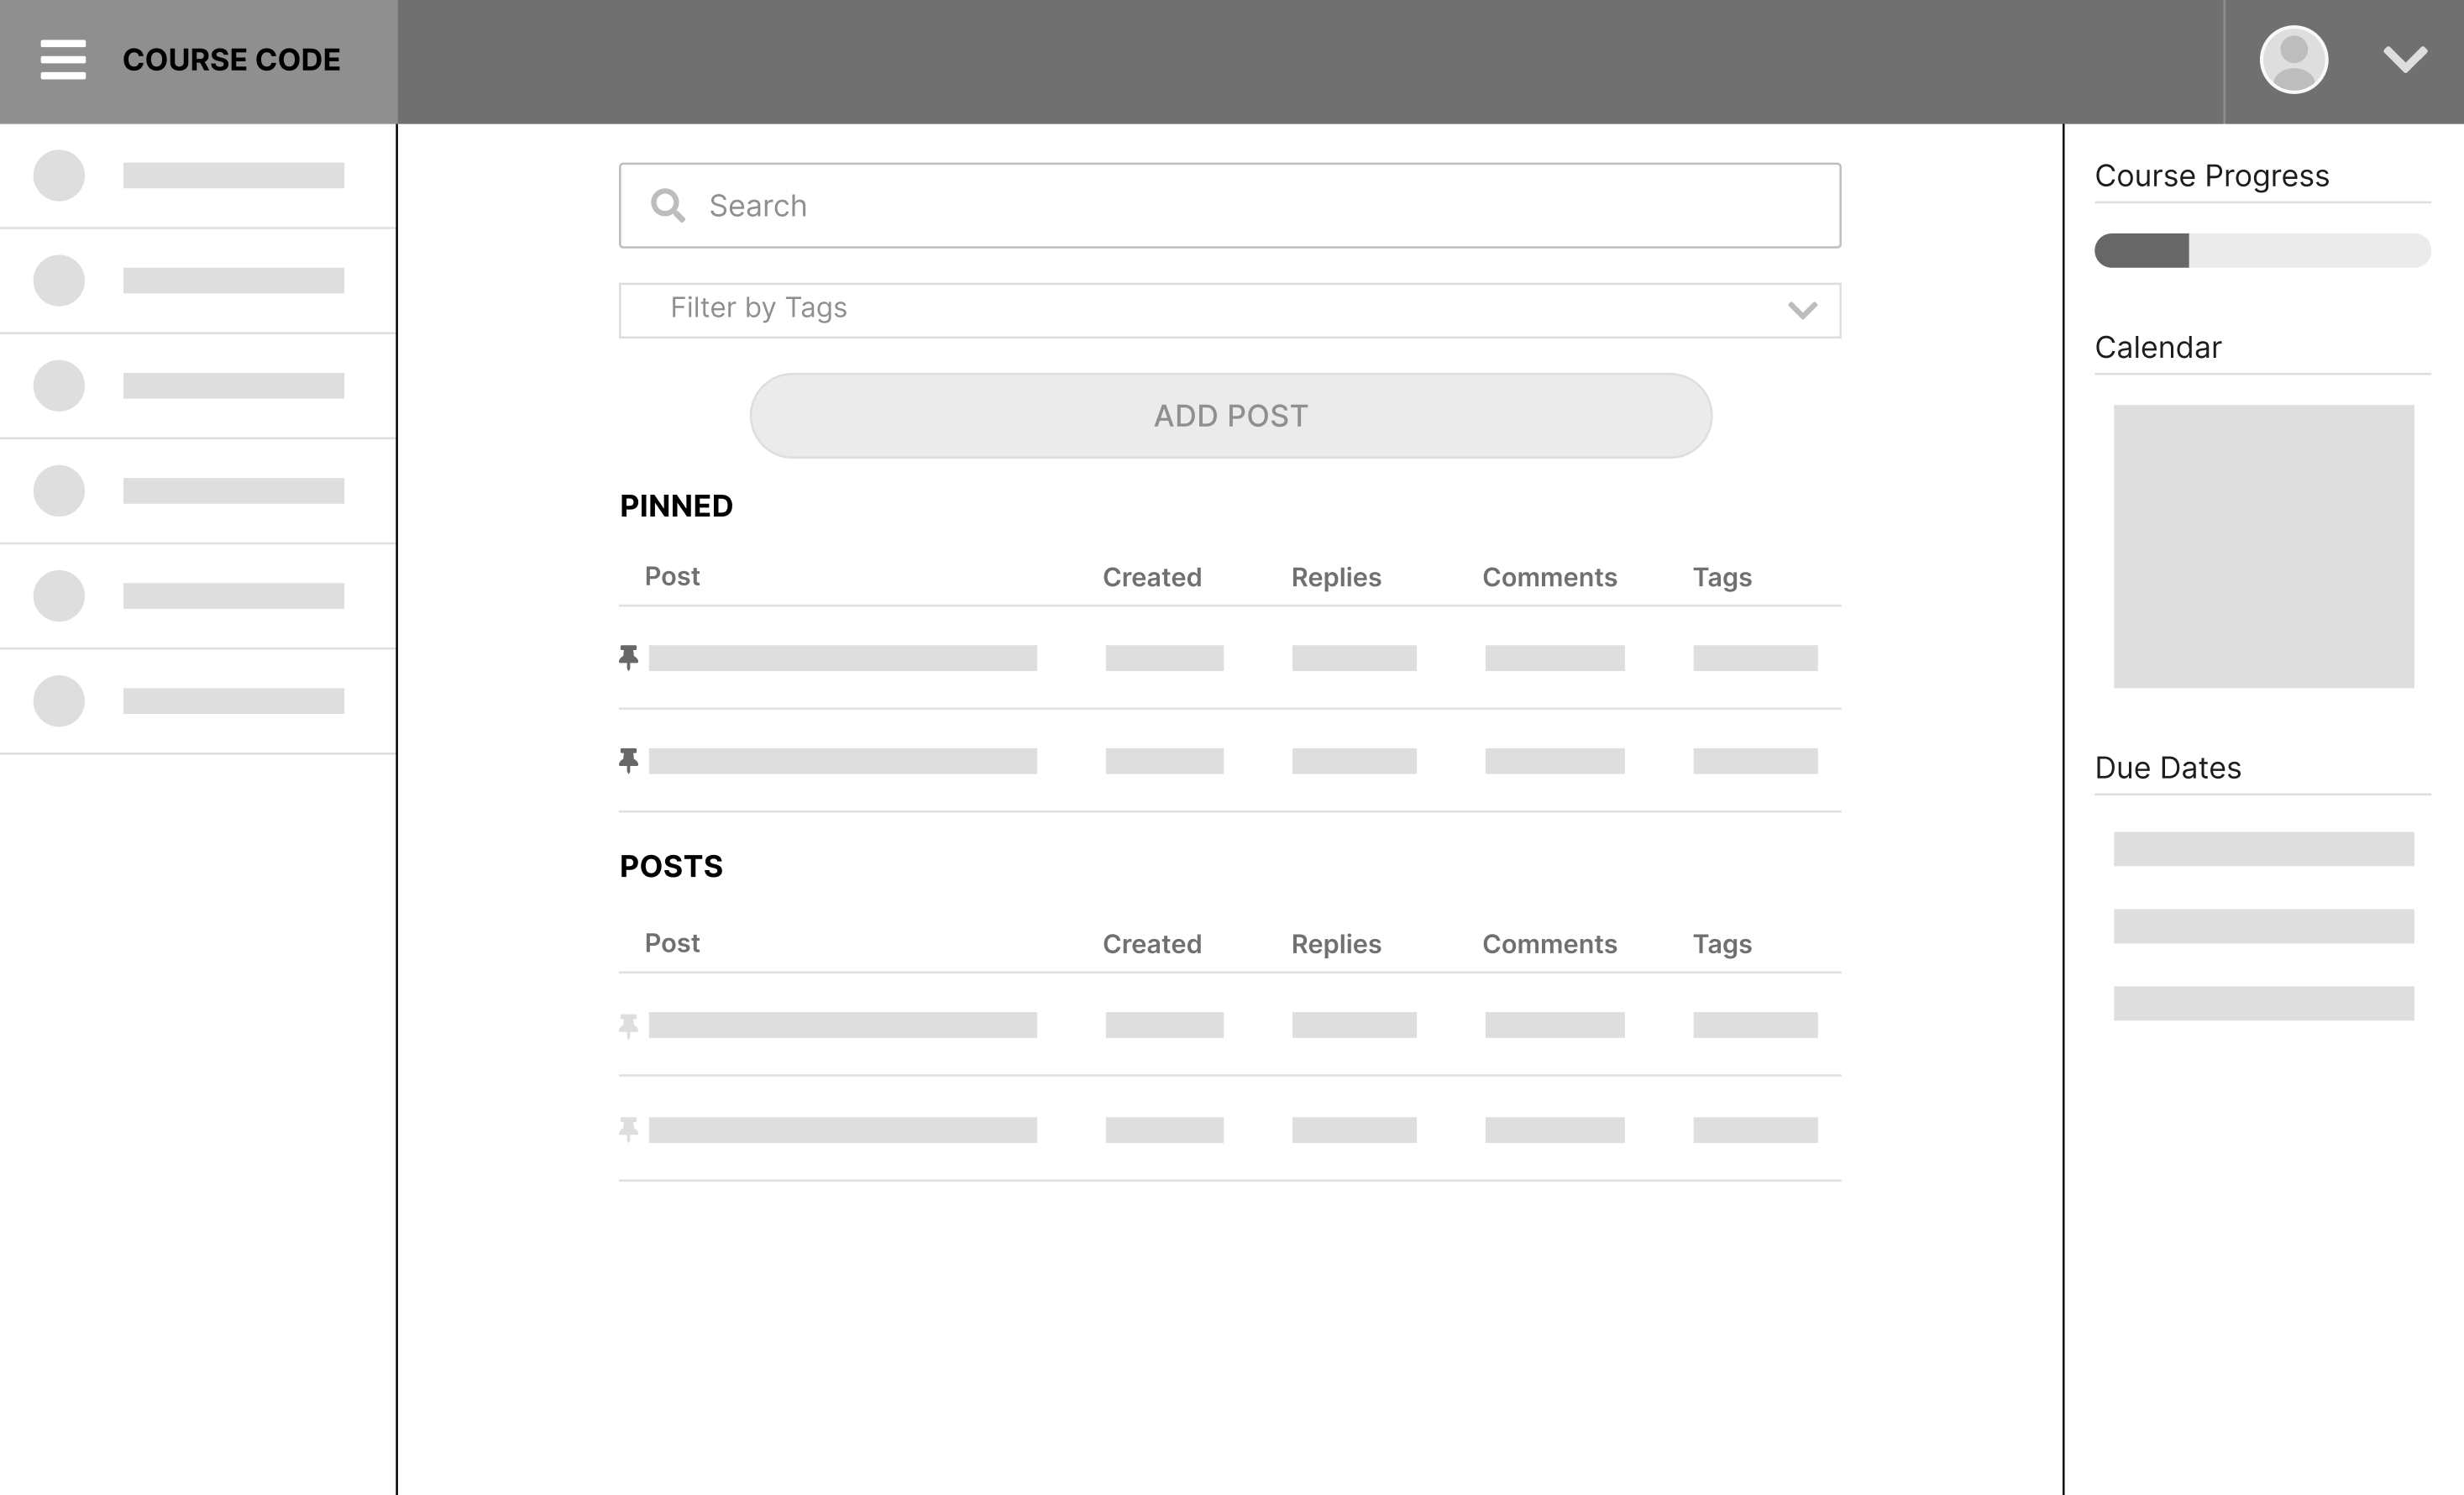
\includegraphics[scale=0.2]{forum-overview-page-admin.png}
    \centering
    \caption{Forum overview page for an admin}
\end{figure}

Admins have an additional button that allows them to pin and unpin posts.

\subsubsection{Post Page}

\begin{figure}[h!]
    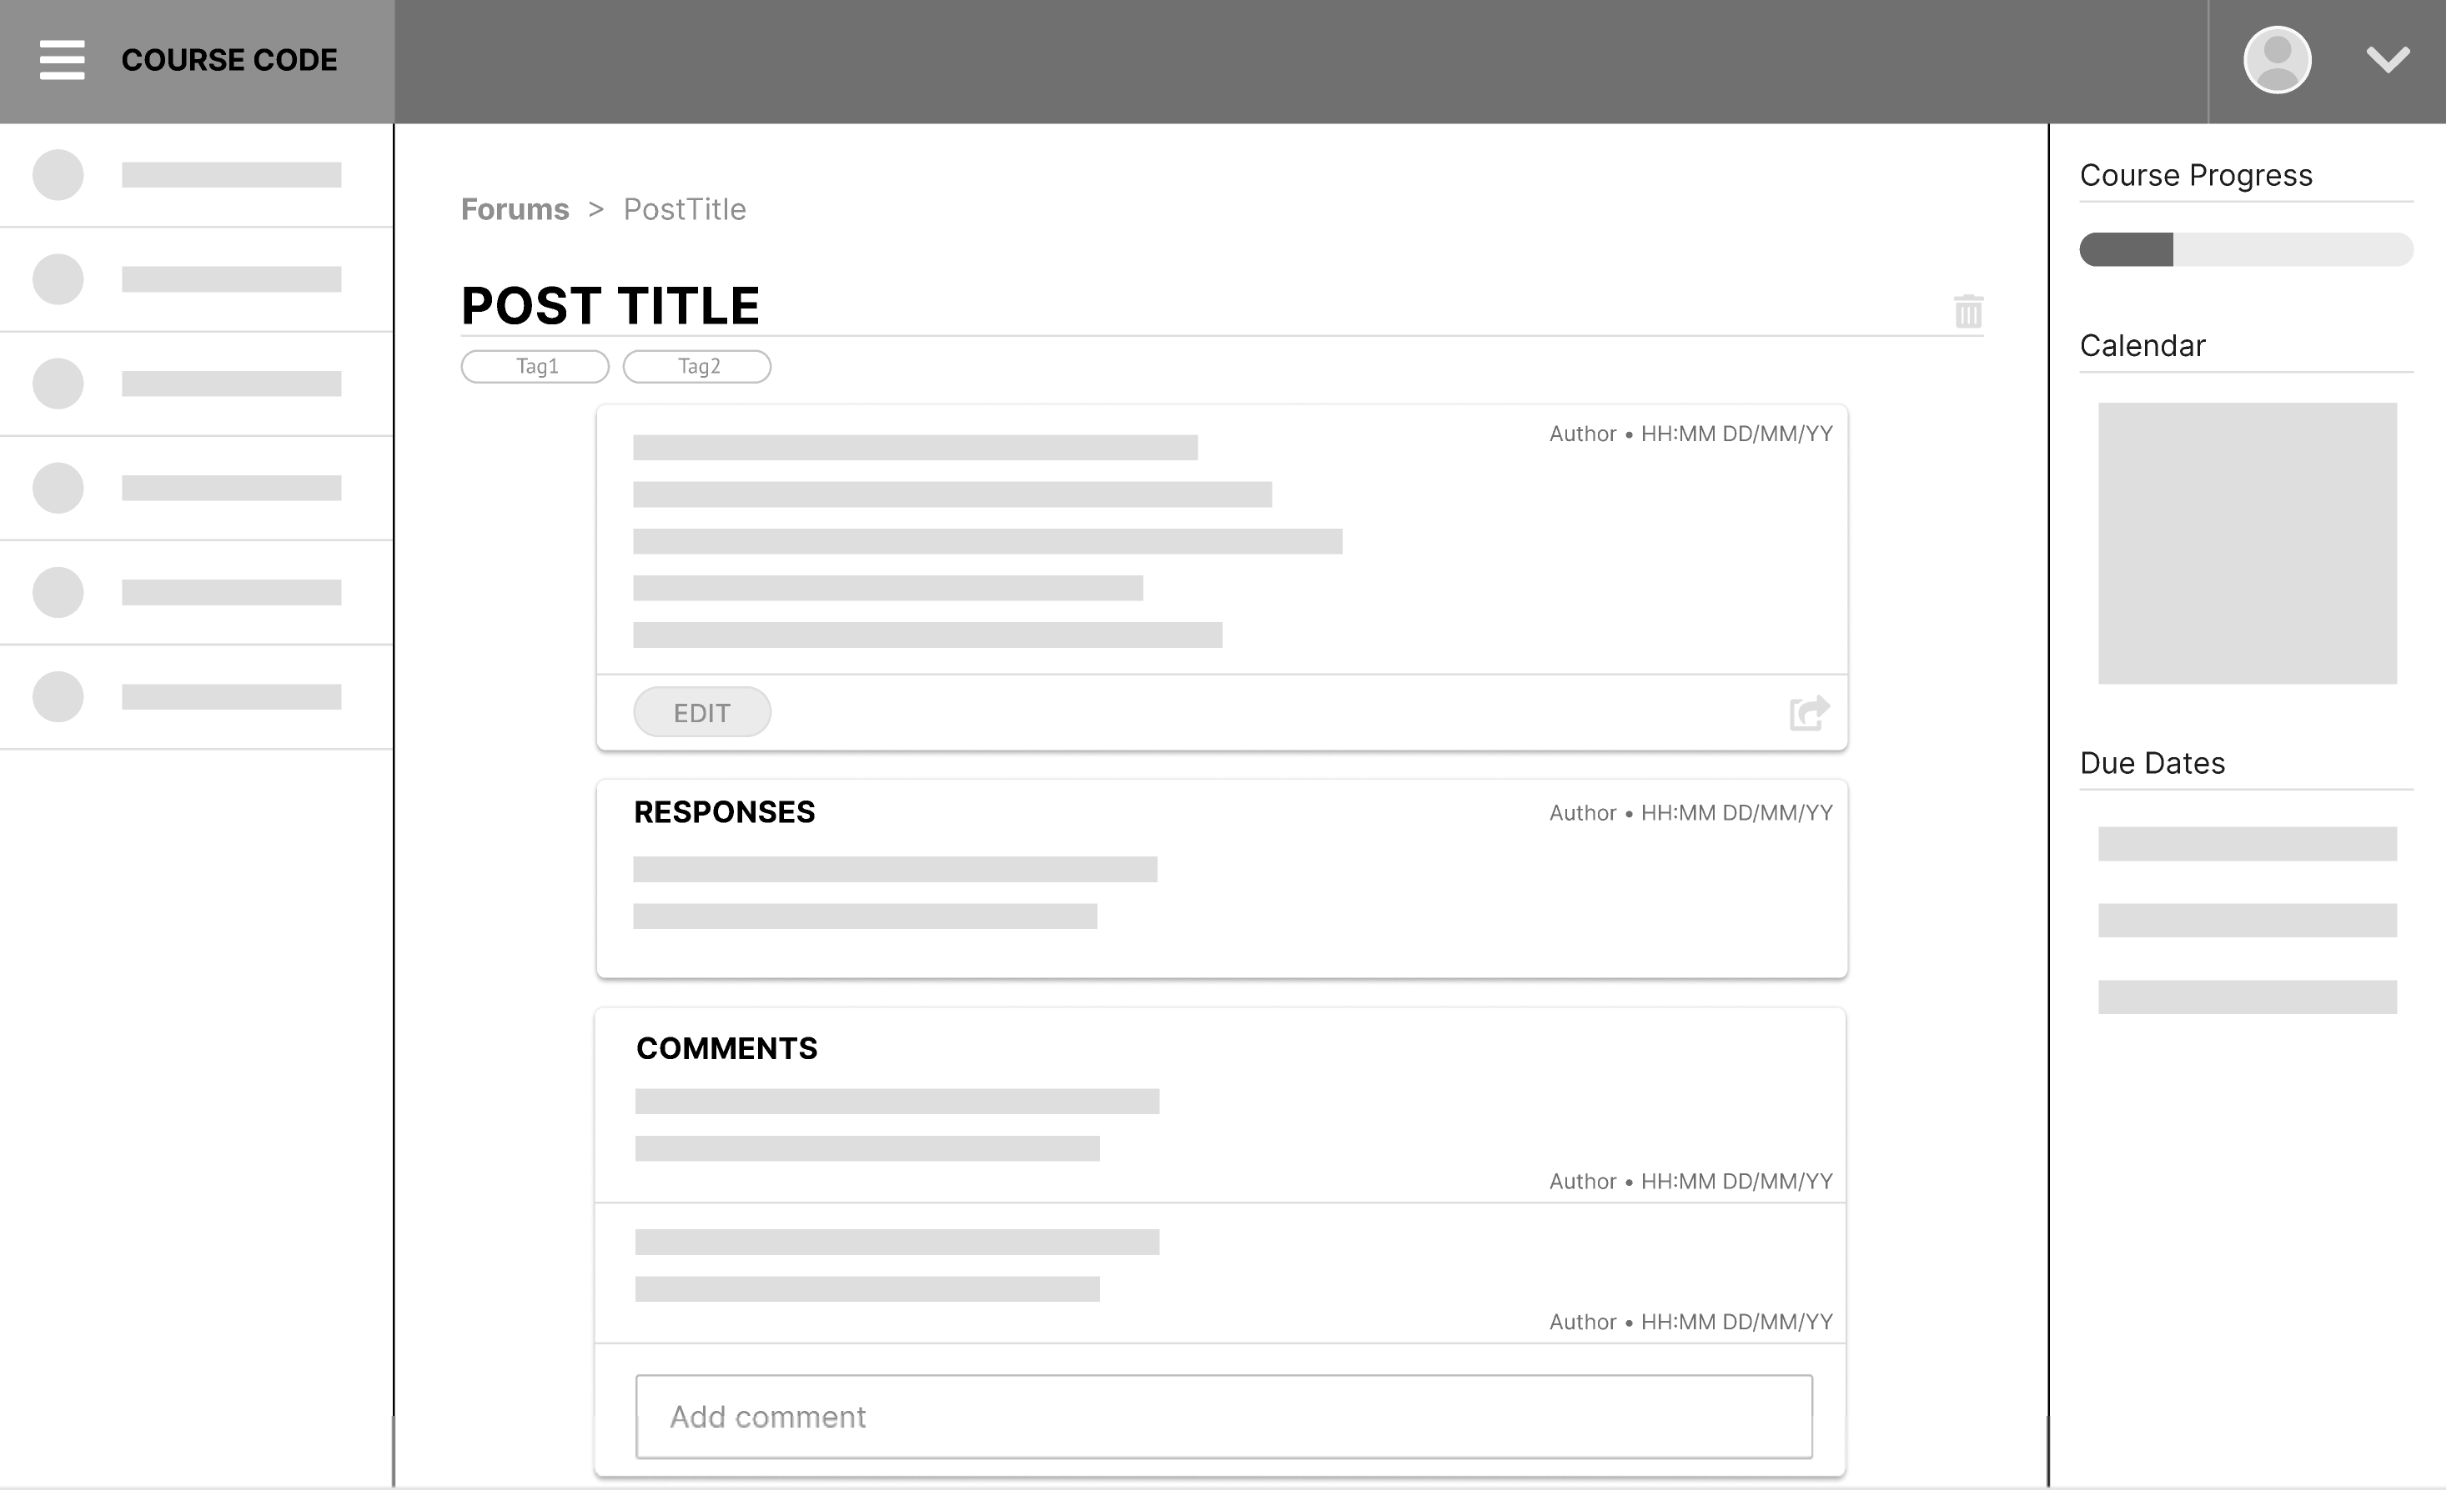
\includegraphics[scale=0.2]{forum-post-page-answered-student.png}
    \centering
    \caption{Forum post page for a student}
\end{figure}

Each forum post has its own post page which contains the post details, responses and comments.
Students are able to edit their posts from the post page if required.
They can easily view the instructor's response, if any, in the responses section.
The comments section allows the author to view and leave any additional comments.
It also gives other students a place to write a response or ask questions based on that forum post.

\begin{figure}[h!]
    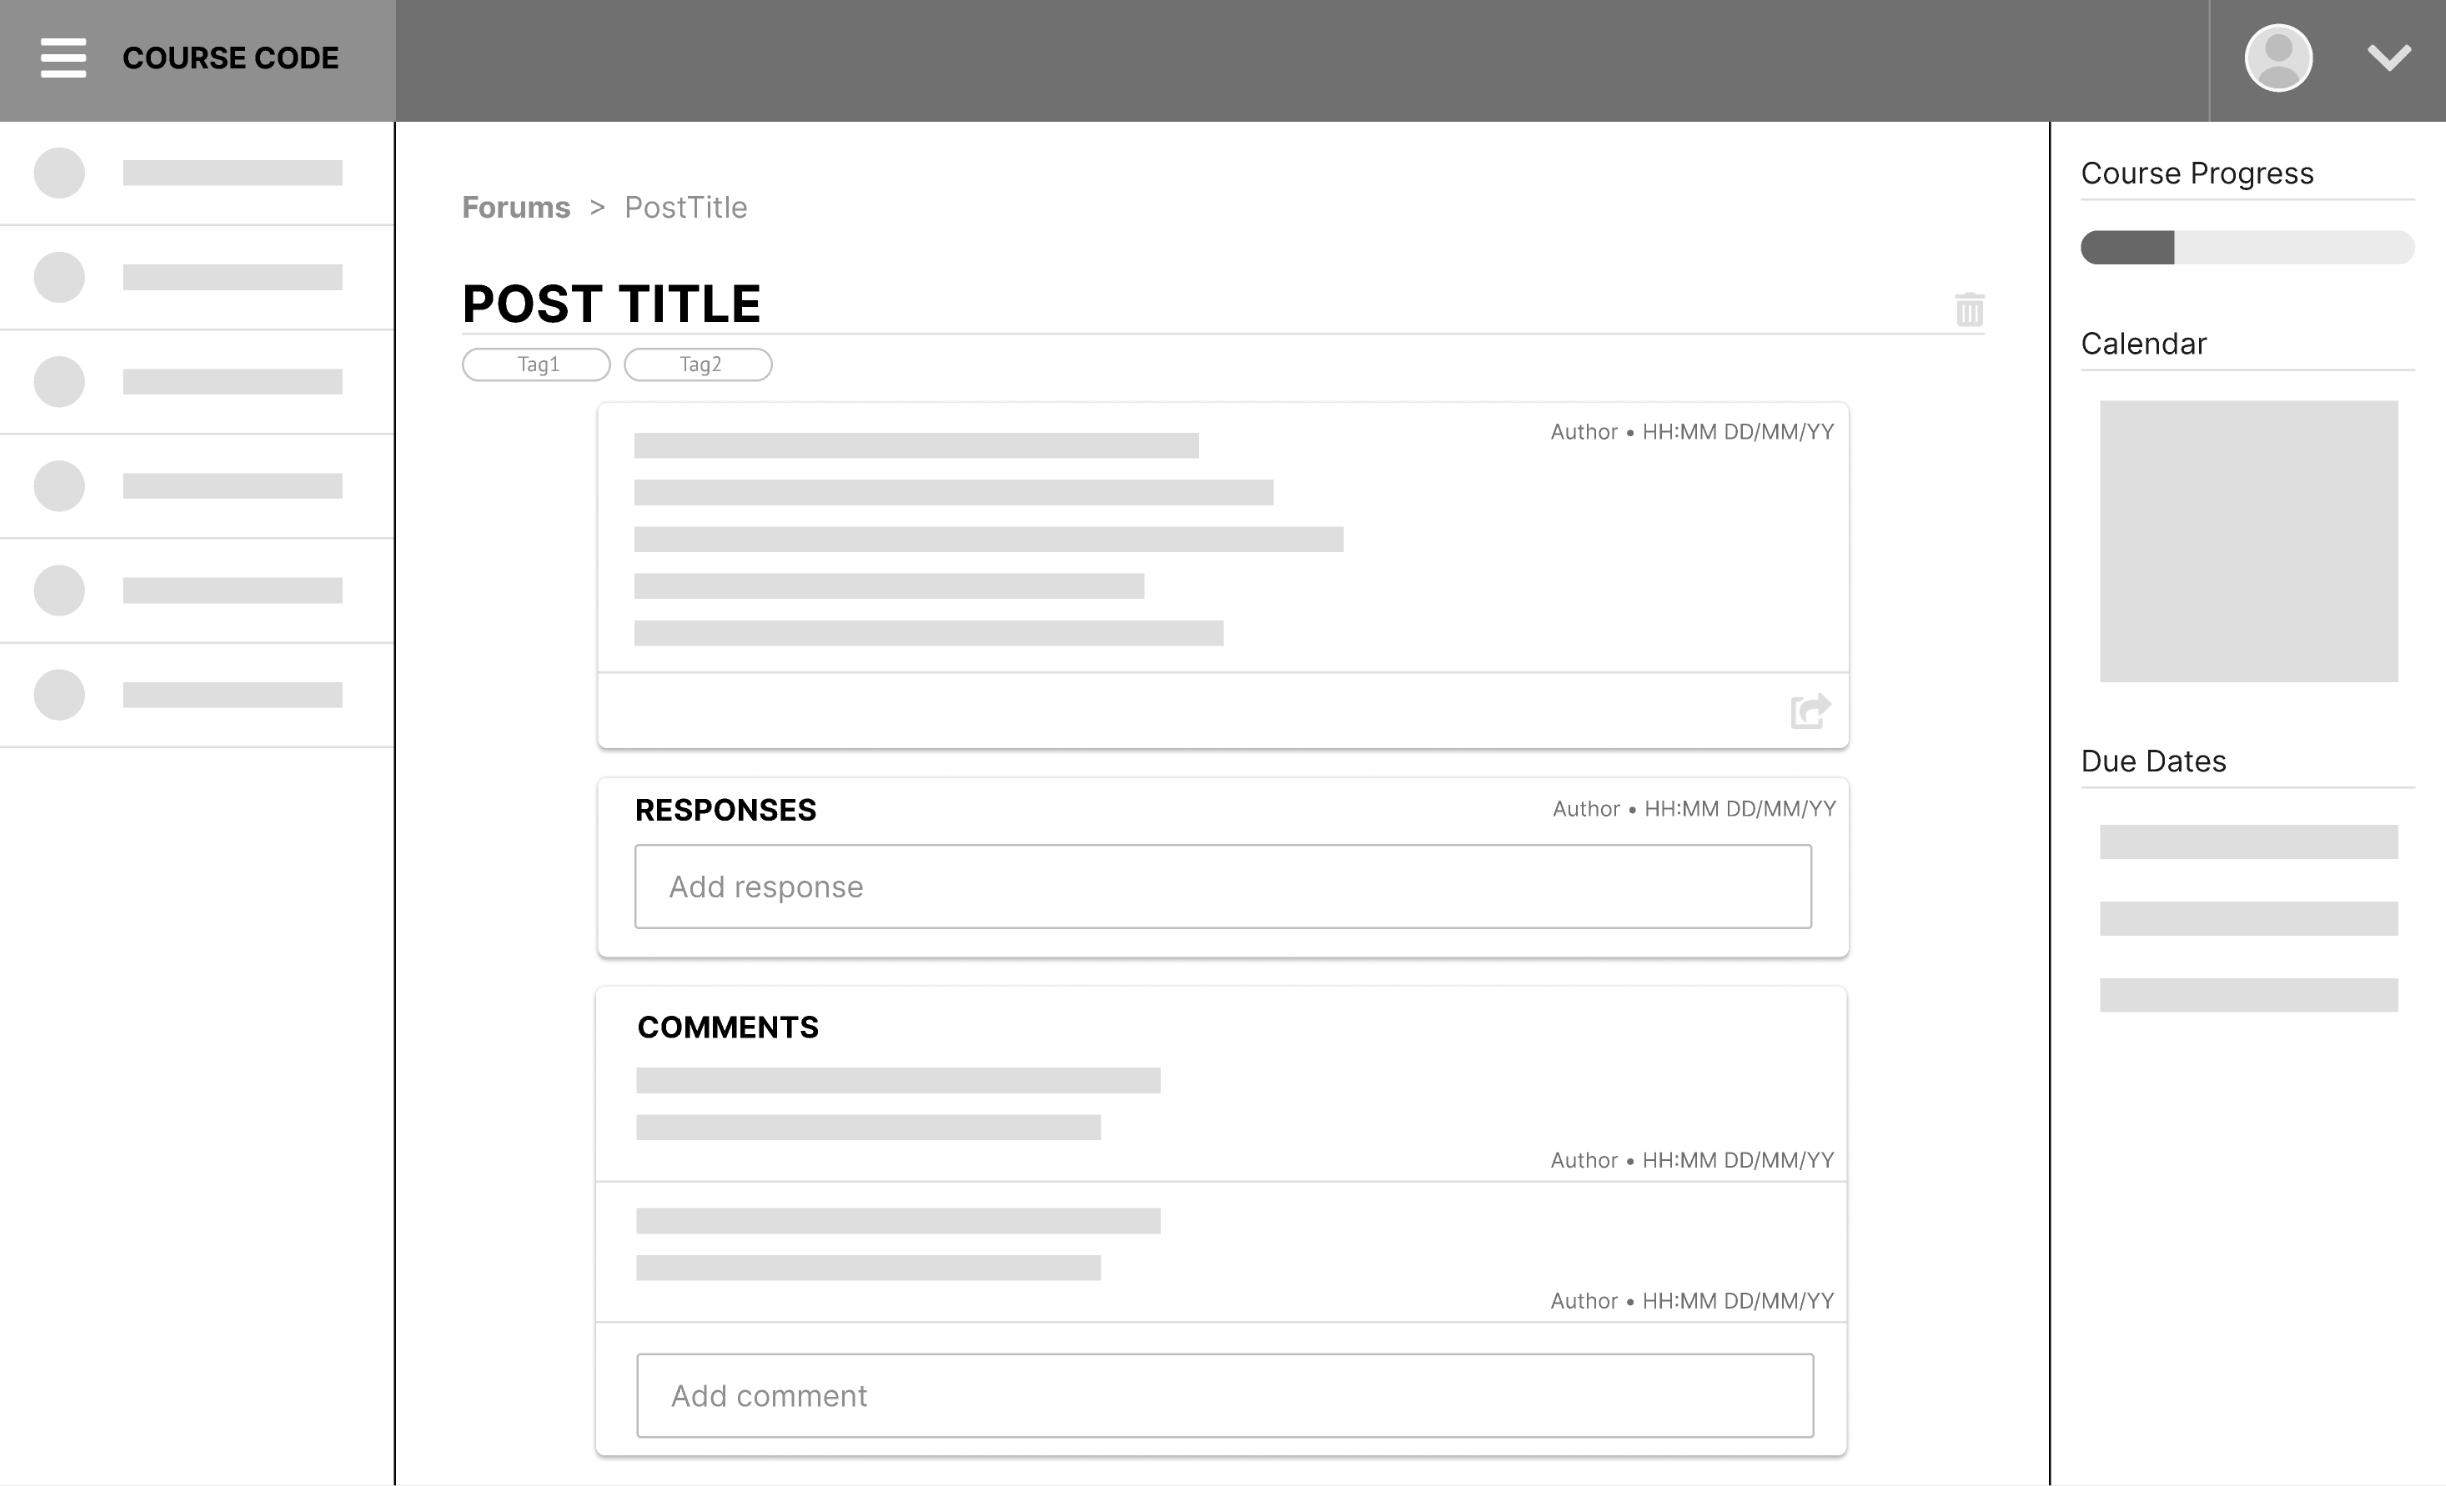
\includegraphics[scale=0.2]{forum-post-page-unanswered-admin.png}
    \centering
    \caption{Forum post page for an admin}
\end{figure}

If a forum post is unanswered, an admin is able to leave a response.
The current idea is to restrict this so that only admins can write responses to ensure that all responses are verified.
It also ensures that forum posts aren't left unanswered if a student accidentally leaves a follow-up question in the responses area, instead of the comments section.
This method of implementation may be reassessed if time allows.

\subsection{Requirements}
The following features are prioritised using the MoSCoW method which assists in identifying the order in which to implement the requirements.
It contains the following categories

\begin{itemize}
    \item \textbf{Must have} - vital features that are critical to the basic functionality of a project
    \item \textbf{Should have} - important features that aren't critical but add to the basic functionality of a project
    \item \textbf{Could have} - desired features that aren't necessary to the overall project but can provide a better user experience
    \item \textbf{Won't have} - low-priority features that likely won't be able to be completed in the given time-frame
\end{itemize}

\subsubsection{Functional Requirements}
\begin{enumerate}
    \item Users can view a list of forum posts (Must have)
    \item Users can make posts to the forum (Must have)
    \item Users can reply to forum posts (Must have)
    \item Users can embed images and links in their posts (Should have)
    \item Users can share forum posts (Should have)
    \item Users can categorise forum posts (Should have)
    \item Users can search forum posts (Should have)
    \item Users can clearly see which posts have been read and actioned (Could have)
    \item Admins can pin important forum posts (Should have)
    \item Admins can link/embed materials to forum posts (Could have)
    \item Admins can curate forum questions into collections (Won't have)
\end{enumerate}

\subsection{Backend Assumptions}
Since the backend for the Meta LMS is being built out independently to the individual features, the following contains a description of the ideal backend design for the forum component.

\subsubsection{Database}
The main database table required for this component is one to store all the forum posts.
This would include all the post details including author, title, description, date created and tags.
It would also need to have a way to keep track of the replies and comments left on the forum post.
This could either be done by having separate tables for replies and comments, or by storing a list of replies and comments within each forum post entry.
For each of the forum posts, the author would need to be linked to a user in the user table of the database.

\subsubsection{API}
In terms of the backend API, the following functionality would be required in order to store, retrieve and update the appropriate data from the database.

\begin{enumerate}
    \item Retrieve a list of all forum posts
    \item Retrieve a list of the pinned posts
    \item Retrieve a list of posts related to search term
    \item Retrieve a list of posts related to filter
    \item Retrieve individual post details for post page (including comments and responses)
    \item Store new post details
    \item Store post responses
    \item Store post comments
    \item Update post details when author edits post
    \item Update response when author edits response
    \item Update pinned post list when admin pins/unpins posts
\end{enumerate}

\subsection{Evaluation}
In order to ensure that the needs of students and educators are met for this forum component, the following evaluation methods will be used.

\subsubsection{Functional Requirements}
The first form of analysis that will be used to evaluate the forum component is to compare the completed product with the functional requirements defined during Thesis A.
This will ensure that all of the essential requirements are covered.
If there is enough time, it will also highlight any lower priority requirements that may be added to the component.

\subsubsection{Usability Testing}
To test the usability of the system, usability tests will be run with various students and educators.
A usability test typically consists of having participants who have never used the system before run through a scenario.
In this case, it may be appropriate to test that a student is able to create and view a post.
Similarly, an admin might be tested to see if they can easily find an unanswered post and respond to it.
Different measures like number of errors and time it takes to complete a task can be used to quantitatively assess the usability of the system.
As a result, usability testing will help to identify any areas of the system that may be confusing or difficult to use.

\subsection{Project Timeline}
Below is a rough guideline of some milestones that should be met throughout the year in order to complete this feature on time.

\subsubsection{Thesis A}
The focus of Thesis A, Term 1 2021, is solely based around researching current learning management systems to get a good understanding of the desired features required for a meta LMS.
It also includes more in-depth research of forums and planning out what this forum component should consist of.

\begin{figure}[h!]
    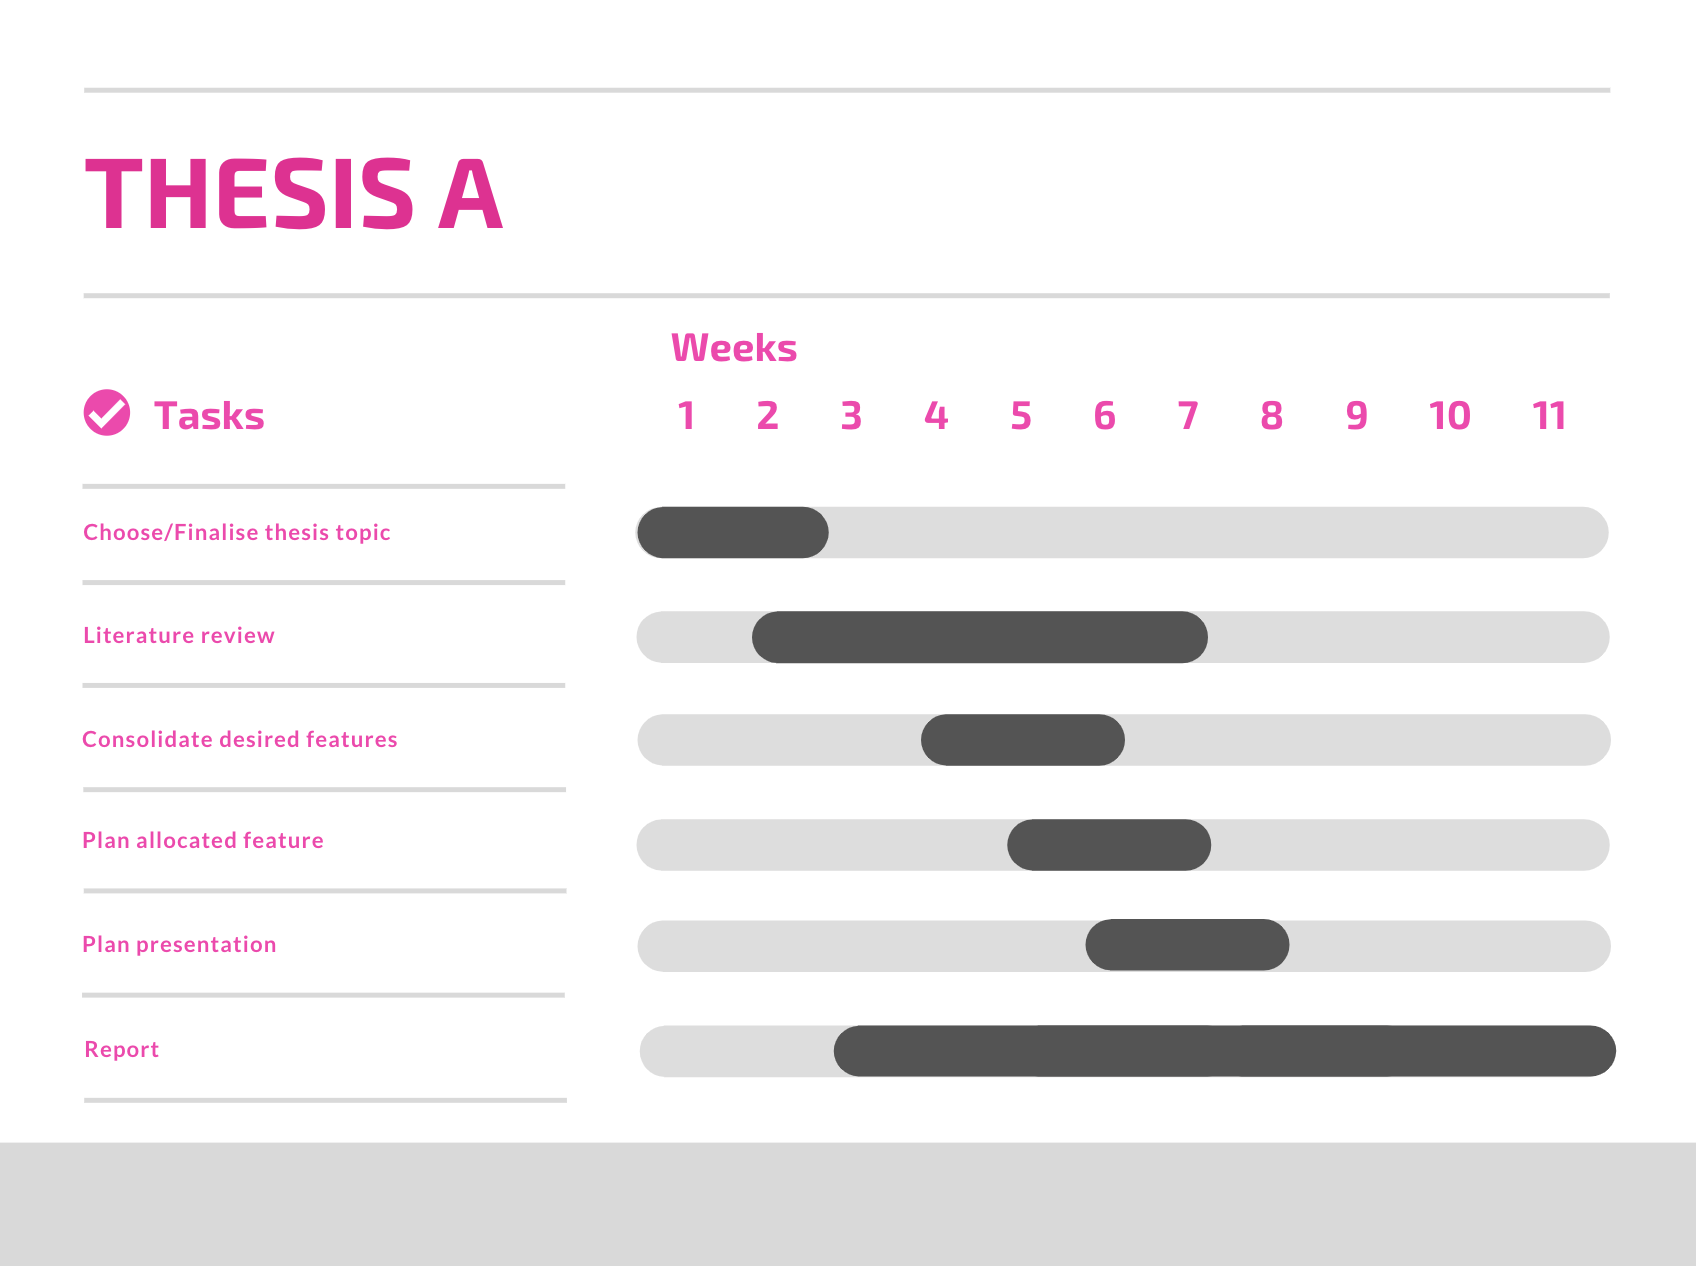
\includegraphics[scale=0.4]{forum-thesis-a.png}
    \centering
    \caption{Thesis A Timeline}
\end{figure}

\newpage

\subsubsection{Thesis B}
Thesis B, Term 2 2021, will hopefully consist of most of the implementation work for forums.
It will start with some market research to get a good understanding of the wants and needs to students and educators.
Analysis of these results will help to finalise the features and designs of the forum component.

Once the frontend and backend designs have been finalised, the forum overview page and post page will be implemented.
This includes viewing posts, making posts and replying to posts.

The next focus is the searching and filtering functionalities.
This includes searching the forum and filtering based on pre-defined tags.

Finally, in Thesis B, the ability to pin and share posts will be added.
This should conclude the implementation of all the main features of the forum component.

\begin{figure}[h!]
    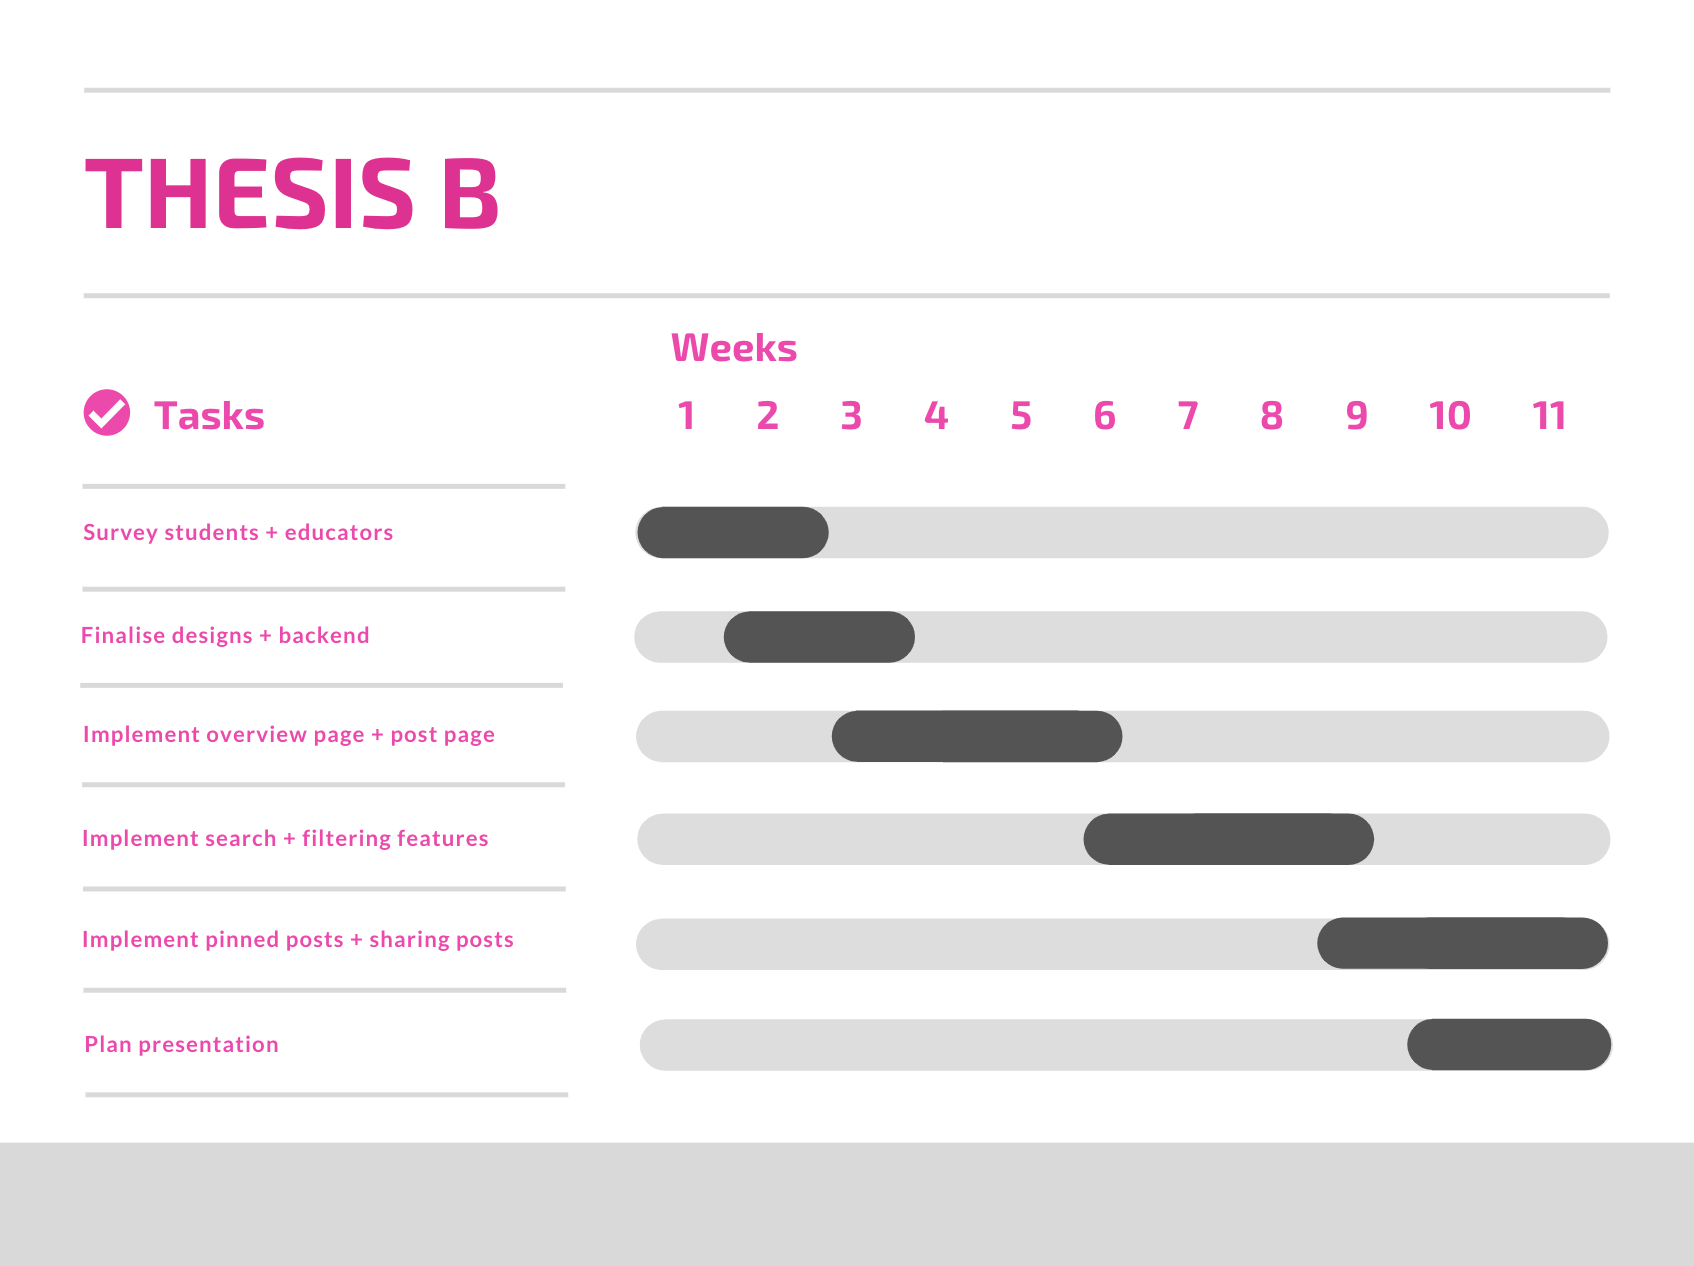
\includegraphics[scale=0.4]{forum-thesis-b.png}
    \centering
    \caption{Thesis B Timeline}
\end{figure}

\subsubsection{Thesis C}
Thesis C, Term 3 2021, is mainly centred around finalising the implementation and evaluating the solution.
The first few weeks will consist of completing any unfinished features, cleaning up the UI and debugging any problems.
If there is time, extra features could be implemented.
Time will also be allocated to integrating the forum with the rest of the LMS.

The middle weeks of the term will focus on analysis and usability testing.
This will help see if the users' needs have been met by the implemented solution.

The final few weeks will consist of any final improvements and testing.
The results from the analysis will help to fix any problems with the forum component.

\begin{figure}[h!]
    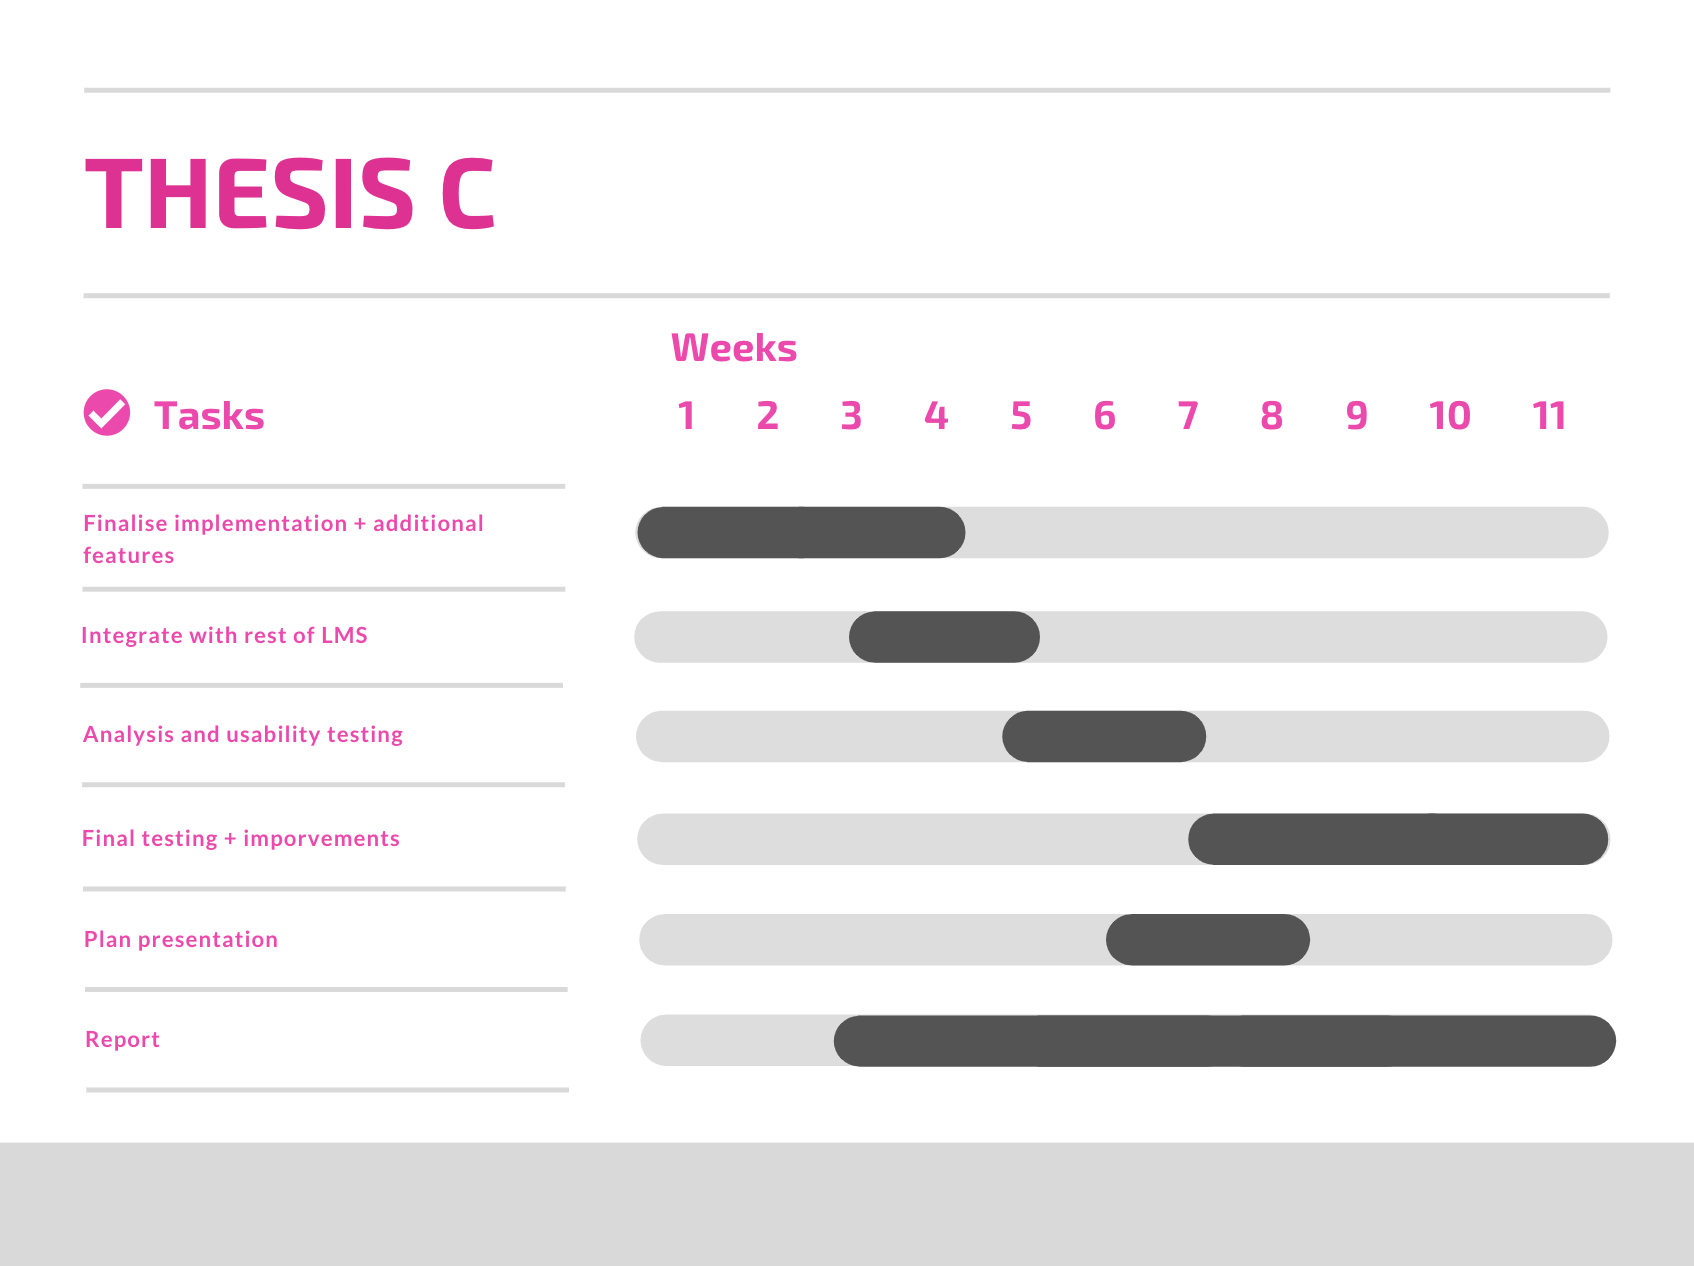
\includegraphics[scale=0.4]{forum-thesis-c.png}
    \centering
    \caption{Thesis C Timeline}
\end{figure}
\section{Assessments}
\subsection{Overview}
The Assessment feature consists of a quiz and poll system where the poll can be used as a supplementary tool for the quiz or to be used as a general poll system. Quizzes are a widely used form of assessing students' knowledge about a particular topic or course. It is beneficial to students as it gives a good indication of their understanding of a topic and whether they need to revise more in a particular area. Likewise, it is beneficial to course lecturers as they'll be able to gauge the students' understanding and whether they should change their teaching methods or revise the content with students to resolve difficulties with concepts. Therefore it is an essential in any learning management system to provide quizzes, which most, if not all, learning management systems do. However, some existing quiz systems lack in providing an aesthetic user interface and useful feedback for both parties. Therefore, the Assessment feature aims at:
\begin{itemize}
    \item allowing quiz submissions and grading to be performed on the same platform for convenience
    \item providing additional useful statistics as feedback to help improve the teachings of a course instructor and the learnings of a student enrolled in the course
    \item having an appealing, readable interface for both course instructors and students
    \item providing a poll system for general poll use or as a means for students to communicate what topic they'd like the course lecturer to revise
\end{itemize}

The core features for quizzes include being able to:
\begin{itemize}
    \item create/remove/edit a question
    \item answer/edit an answer to a question
    \item choose between three types of questions to create:
    \begin{itemize}
    	\item multiple choice - select one answer only
    	\item short answer
    	\item checkboxes - select none, one or multiple answers
    \end{itemize}
    \item auto-save and manual save answers during quiz attempt
    \item timer that runs during quiz attempt
\end{itemize}

\begin{figure}[h!]
	\centering
	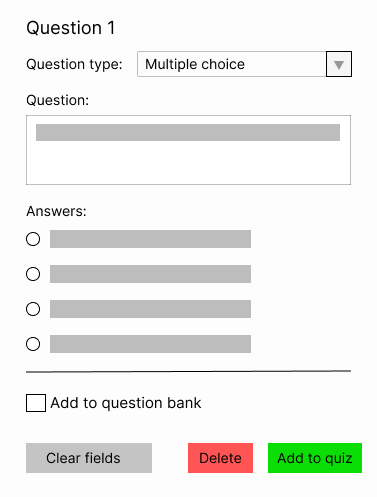
\includegraphics[scale=0.4]{assessments-quiz-creation}
	\caption{Quiz creation (Instructor's view)}
\end{figure}

\begin{figure}[h!]
\centering
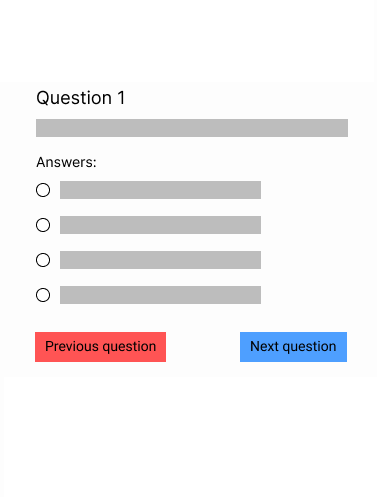
\includegraphics[scale=0.4]{assessments-quiz-usage}
\caption{Quiz usage (Student's view)}
\end{figure}

The core features for polls include being able to:
\begin{itemize}
	\item create/remove a poll
	\item create/remove/edit a poll option
	\item select poll options/s to vote and change your vote
	\item choose between two types of polls to create:
		\begin{itemize}
			\item restricted - can only vote for 1 option
			\item open - can vote for multiple options
		\end{itemize}
\end{itemize}


\subsection{Stakeholders}
\begin{itemize}
	\item Course lecturers
	\item Admins
	\item Students
\end{itemize}

\subsection{Functional Requirements}
The list of functional requirements' priority level will be determined using the MoSCoW method to clearly outline what needs to be implemented throughout the thesis and what the minimum viable product should have. 

The MoSCoW method splits requirements based on 4 categories:
\begin{itemize}
	\item \textcolor{Red}{Must Have}
	\item \textcolor{Blue}{Should Have}
	\item \textcolor{Orange}{Could Have}
	\item \textcolor{Green}{Won't Have}
\end{itemize}

A requirements survey was conducted and completed by me and other Thesis A students to gauge what was the priorities for each requirement. The results for the Assessment feature from the survey and my own ideas were combined to form the following functional requirements:

\subsubsection{Quiz creation}
\begin{enumerate}
	\item Course lecturers can create a quiz \textcolor{Red}{[Must Have]}
	\item Course lecturers can add questions to a quiz \textcolor{Red}{[Must Have]}
	\item Course lecturers can create different types of quiz questions (multiple-choice, short answer, checkboxes) \textcolor{Red}{[Must Have]}
	\item Course lecturers can set up a timer or due date for a quiz \textcolor{Red}{[Must Have]}
	\item Course lecturers can add "drag and drop" type questions \textcolor{Orange}{[Could Have]}
	\item Course lecturers can add "connect the pairs" type questions \textcolor{Orange}{[Could Have]}
	\item Course lecturers can add media (audio or  video) into a question as the entire question or as a supplementary material to the question \textcolor{Orange}{[Could Have]}
	\item Course lecturers can create a question bank \textcolor{Blue}{[Should Have]}
	\item Course lecturers can add a question to a question bank \textcolor{Blue}{[Should Have]}
	\item Course lecturers can import a question from a question bank \textcolor{Blue}{[Should Have]}
\end{enumerate}

\subsubsection{Quiz modification/removal}
\begin{enumerate}
	\item Course lecturers can edit/remove a quiz \textcolor{Red}{[Must Have]}
	\item Course lecturers can edit/remove a question \textcolor{Red}{[Must Have]}
	\item Course lecturers can remove a question bank \textcolor{Blue}{[Should Have]}
	\item Course lecturers can remove a question from a question bank \textcolor{Blue}{[Should Have]}
\end{enumerate}

\subsubsection{Quiz usage}
\begin{enumerate}
	\item Students can answer a quiz question \textcolor{Red}{[Must Have]}
	\item Students can edit any of their answers during the quiz \textcolor{Red}{[Must Have]}
	\item Students can submit a quiz attempt \textcolor{Red}{[Must Have]}
	\item Students can manually save their progress at any time \textcolor{Blue}{[Should Have]}
\end{enumerate}

\subsubsection{Poll creation}
\begin{enumerate}
	\item Course lecturers can create different types of polls (can vote either 1 option only or multiple options) \textcolor{Red}{[Must Have]}
	\item Course lecturers can add an option to a poll \textcolor{Red}{[Must Have]}
\end{enumerate}

\subsubsection{Poll modification/closing}
\begin{enumerate}
	\item Course lecturers can edit/remove options \textcolor{Red}{[Must Have]}
	\item Course lecturers can close polls \textcolor{Red}{[Must Have]}
	\item Course lecturers can set a poll closing date \textcolor{Blue}{[Should Have]}
	\item Course lecturers can close a poll but make results viewable \textcolor{Orange}{[Could Have]}
\end{enumerate}

\subsubsection{Poll usage}
\begin{enumerate}
	\item Students can vote for one or multiple options (depending on poll type) \textcolor{Red}{[Must Have]}
	\item Students can add an option (if course lecturer enables the option for it) \textcolor{Orange}{[Could Have]}
\end{enumerate}

\subsubsection{Viewing quiz results and feedback}
\begin{enumerate}
	\item Students can view results against their answers \textcolor{Blue}{[Should Have]}
	\item Students, course lecturers and admins can see how many students selected each answer for a question \textcolor{Blue}{[Should Have]}
	\item Students can view topic or lecture the question derives from \textcolor{Blue}{[Should Have]}
	\item Students can view an explanation of the correct answer if the question is answered incorrectly \textcolor{Orange}{[Could Have]}
\end{enumerate}

\subsubsection{Re-usability}
\begin{enumerate}
	\item Course lecturers can add a question to a general question bank \textcolor{Blue}{[Should Have]}
	\item Course lecturers can import/export quizzes \textcolor{Blue}{[Should Have]}
	\item Course lecturers can import/export questions \textcolor{Blue}{[Should Have]}
\end{enumerate}


\subsection{Non-functional Requirements}
The non-functional requirements used is heavily inspired by the Jakob Nielsen's 10 usability heuristics that's used to evaluate the usability of user interfaces. 

\begin{enumerate}
	\item \textbf{Efficiency} - users are able to perform tasks without taking too many steps
	\item \textbf{Learnability} - new and returning users are able to quickly learn how to use and interact with the feature on the go
	\item \textbf{Performance} - operations within the feature are completed within a timely manner, resulting in a smooth process
	\item \textbf{Consistency} - components, colour themes and formats are consistent across pages 
	\item \textbf{Aesthetic and minimalist design} - the user interface is appealing and simple while providing the expected features
	\item \textbf{Re-usability} - users are able to re-use components and content they've previously made
\end{enumerate}


\section{Required Training/Upskilling}
Training across multiple areas will be required in order to develop the Learning Management System:

\begin{itemize}
	\item Create technical diagrams using Miro (diagramming tool)
	\item Develop React skills
	\item Explore and experiment with graph visualisation libraries (to display statistics)
	\item Research SCORM and other standards used in learning management systems
\end{itemize}

\section{Assumptions}
\subsection{Back-end Assumptions}
The following back-end assumptions contains details of the final backend technologies used, as discussed with other Thesis A students, and general assumption of the database which data will be retrieved from via API calls. 

\subsubsection{Technologies Used}
The technologies that will be used are:
\begin{itemize}
	\item Back-end runtime environment: Node.js
	\item Web application framework: Express.js
	\item Database management system: PostgreSQL
\end{itemize}

\subsubsection{Database}
The use of a relational database will be ideal as it'll be more organised and querying for particular data related to each other will be easier during the implementation of the Assessment feature. 

Potential tables involved would include a Question, Poll, Quiz and User table. 


\subsection{Front-end Assumptions}
The following front-end assumptions contains details of the final front-end technologies used, as discussed with other Thesis A students, and a breakdown of the Assessment feature to give a better insight of the implementation process.

\subsubsection{Technologies Used}
The technologies that will be used are:
\begin{itemize}
	\item Web application framework: React
	\item Component library for React: Material UI
\end{itemize}

\subsubsection{Feature Breakdown}
Since the React frameworks structures content into re-usable, isolated components, the Assessment feature will need to be broken down into such components. Below are the main components that will likely be implemented during Term 2:
\begin{itemize}
	\item Question
	\item Quiz
	\item Poll Option
	\item Poll
	\item Timer
	\item Question Bank
	\item Quiz Results
	\item Answer Explanation
\end{itemize}


\section{Timeline}
\subsection{Term 1 (Thesis A)}
Term 1 will mainly focus on literature research, outlining the main and potential features required to achieve the goals of this thesis.\\

\begin{figure}[h!]
	\centering
	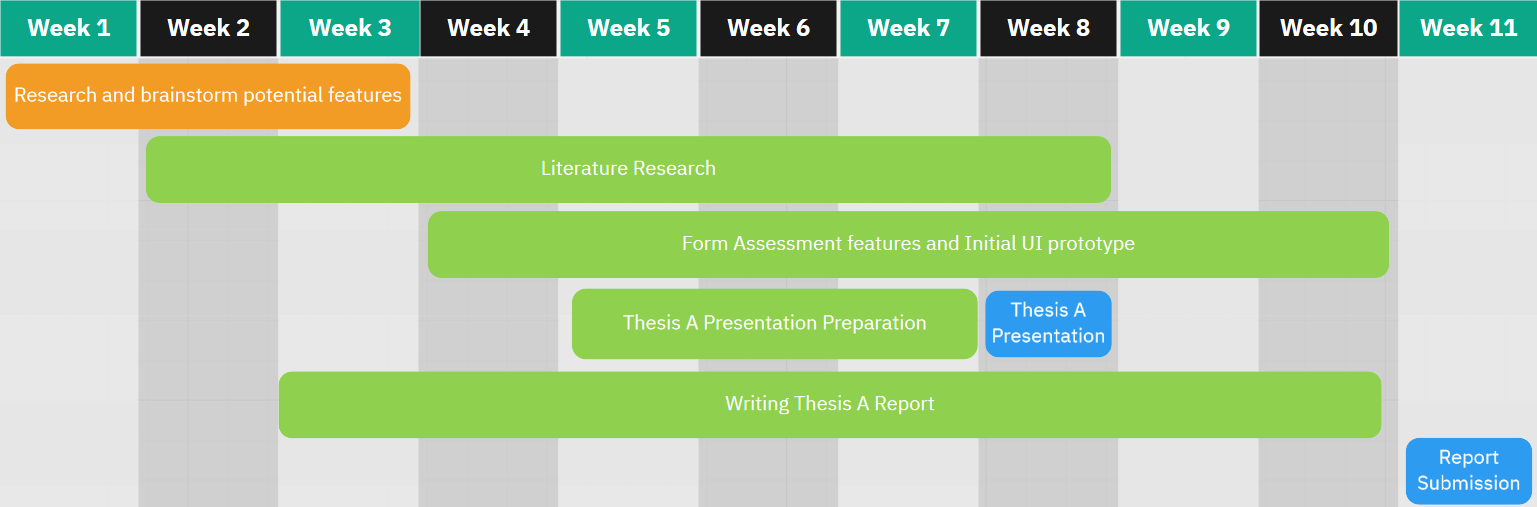
\includegraphics[scale=0.4]{assessments-thesis-a}
	\caption{Thesis A Timeline}
\end{figure}

\subsection{Term 2 (Thesis B)}
Term 2 will mainly focus on implementation of the core features and ensuring a good design overall before adding any extra features.\\

\begin{figure}[h!]
	\centering
	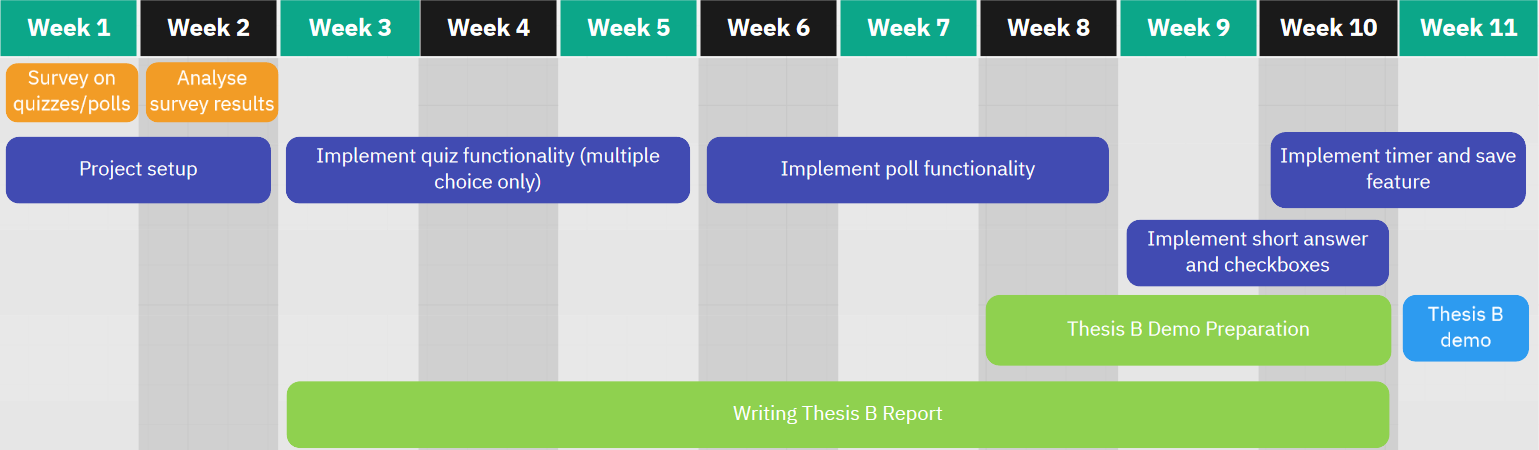
\includegraphics[scale=0.4]{assessments-thesis-b}
	\caption{Thesis B Timeline}
\end{figure}

\subsection{Term 3 (Thesis C)}
Term 3 will focus on improving the system based on feedback, implementing additional features and doing a final testing on the system to ensure it satisfies requirements.\\

\begin{figure}[h!]
	\centering
	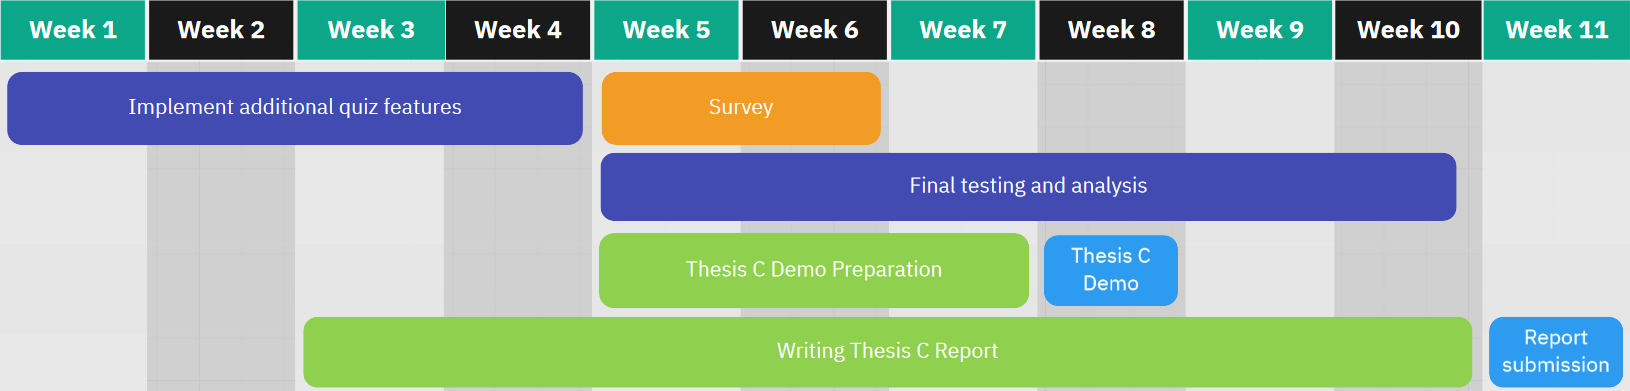
\includegraphics[scale=0.38]{assessments-thesis-c}
	\caption{Thesis C Timeline}
\end{figure}


\subsection{Evaluation}
The system will be evaluated based on:
\begin{itemize}
	\item \textbf{Functional requirements} - what was completed, with the satisfactory being all "Must Haves" and some "Should Haves"
	\item \textbf{Non-functional requirements} - whether it satisfies the goals of the feature and performs operations in a timely manner
	\item \textbf{Usability tests} - if users can navigate through the feature and be able to complete operations within the feature
\end{itemize}
